% =============================================================================
%  SLIDE THUYẾT TRÌNH — Dự đoán Sụp đổ Crypto bằng LLM + TRR
%  Biên dịch: xelatex slides.tex   (Font: Noto Sans)
% =============================================================================
\documentclass[10pt,aspectratio=169]{beamer}

%% -------- Packages ----------------------------------------------------------
\usepackage{fontspec}
\usepackage{polyglossia}
\setdefaultlanguage{vietnamese}
\usepackage{tikz}
\usetikzlibrary{shapes,arrows,positioning,calc}
\usepackage{bookmark}
\usepackage{tabularx}
\usepackage{makecell}
\usepackage{hyperref}

%% -------- Metropolis theme --------------------------------------------------
\usetheme[subsectionpage=progressbar]{metropolis}
\metroset{block=fill, numbering=fraction}

\definecolor{cgreen}{HTML}{16a34a}
\definecolor{cgreenlight}{HTML}{22c55e}
\definecolor{cred}{HTML}{dc2626}
\definecolor{cgray}{HTML}{475569}
\definecolor{cbg}{HTML}{f8fafc}

\setbeamercolor{normal text}{fg=black!87}
\setbeamercolor{frametitle}{bg=cgreen, fg=white}
\setbeamercolor{title}{fg=cgreen}
\setbeamercolor{progress bar}{fg=cgreen, bg=cgreen!20}
\setbeamercolor{alerted text}{fg=cred}
\setbeamercolor{example text}{fg=cgreen}
\setbeamercolor{block title}{bg=cgreen, fg=white}
\setbeamercolor{block body}{bg=cbg}
\setbeamercolor{itemize item}{fg=cgreen}
\setbeamercolor{enumerate item}{fg=cgreen}

%% -------- Fonts -------------------------------------------------------------
\setmainfont{Noto Sans}[Scale=1.0]
\setsansfont{Noto Sans}[Scale=1.0]
\setmonofont{DejaVu Sans Mono}[Scale=0.82]

%% -------- Macros ------------------------------------------------------------
\newcommand{\red}[1]{\textcolor{cred}{\textbf{#1}}}
\newcommand{\green}[1]{\textcolor{cgreen}{\textbf{#1}}}
\newcommand{\num}[1]{\textcolor{cred}{\textbf{#1}}}

% =============================================================================
\begin{document}

%% ===== SLIDE 1: BÌA =========================================================
{
\setbeamercolor{background canvas}{bg=white}
\begin{frame}[plain]
  \centering
  \vspace{2.5cm}
  {\fontsize{22}{28}\selectfont\color{cgreen}
   DỰ ĐOÁN SỤP ĐỔ GIÁ CRYPTO BẰNG \\
   SUY LUẬN QUAN HỆ--THỜI GIAN CỦA LLM}
  \vspace{0.5cm}

  {\large Đồ án Big Data $\cdot$ \texttt{arXiv:2410.17266}}
  \vspace{1cm}

  {\small
  \textbf{Nhóm:} [TÊN NHÓM] \quad
  \textbf{Thành viên:} [TÊN] \\
  \textbf{GVHD:} [TÊN GV] \quad [HỌC KỲ/NĂM]
  }
  \vfill

  \begin{tikzpicture}[remember picture, overlay]
    \fill[cgreen!80] (current page.south west) rectangle ([yshift=0.7cm]current page.south east);
    \node[white, font=\footnotesize] at (current page.south)
      {LLM $\to$ tin tức $\to$ cảnh báo sụp đổ $\cdot$ Big Data Pipeline};
  \end{tikzpicture}
\end{frame}
}

%% ===== SLIDE 2: VẤN ĐỀ =====================================================
\begin{frame}{Vấn đề \& Động lực}
  \begin{columns}[T]
    \column{0.55\textwidth}
    \begin{itemize}
      \item Thị trường crypto: \textbf{khối lượng lớn, tốc độ cao, đa dạng}
      \item \alert{Dự đoán hướng giá} $\approx$ bất khả thi (EMH yếu)
        \quad AUROC h=1: \num{0,499}
      \item \green{Rủi ro sụp đổ (crash)} -- có tín hiệu từ tin tức
      \item $|r|$ autocorr(1) = $+0,20$ (volatility clusters)
      \item 19\% biến động trong 5\% ngày lớn nhất
    \end{itemize}
    \vspace{0.3cm}
    \begin{exampleblock}{Mục tiêu}
      Cảnh báo sớm rủi ro -- advisory cho nhà đầu tư
    \end{exampleblock}

    \column{0.42\textwidth}
    \centering
    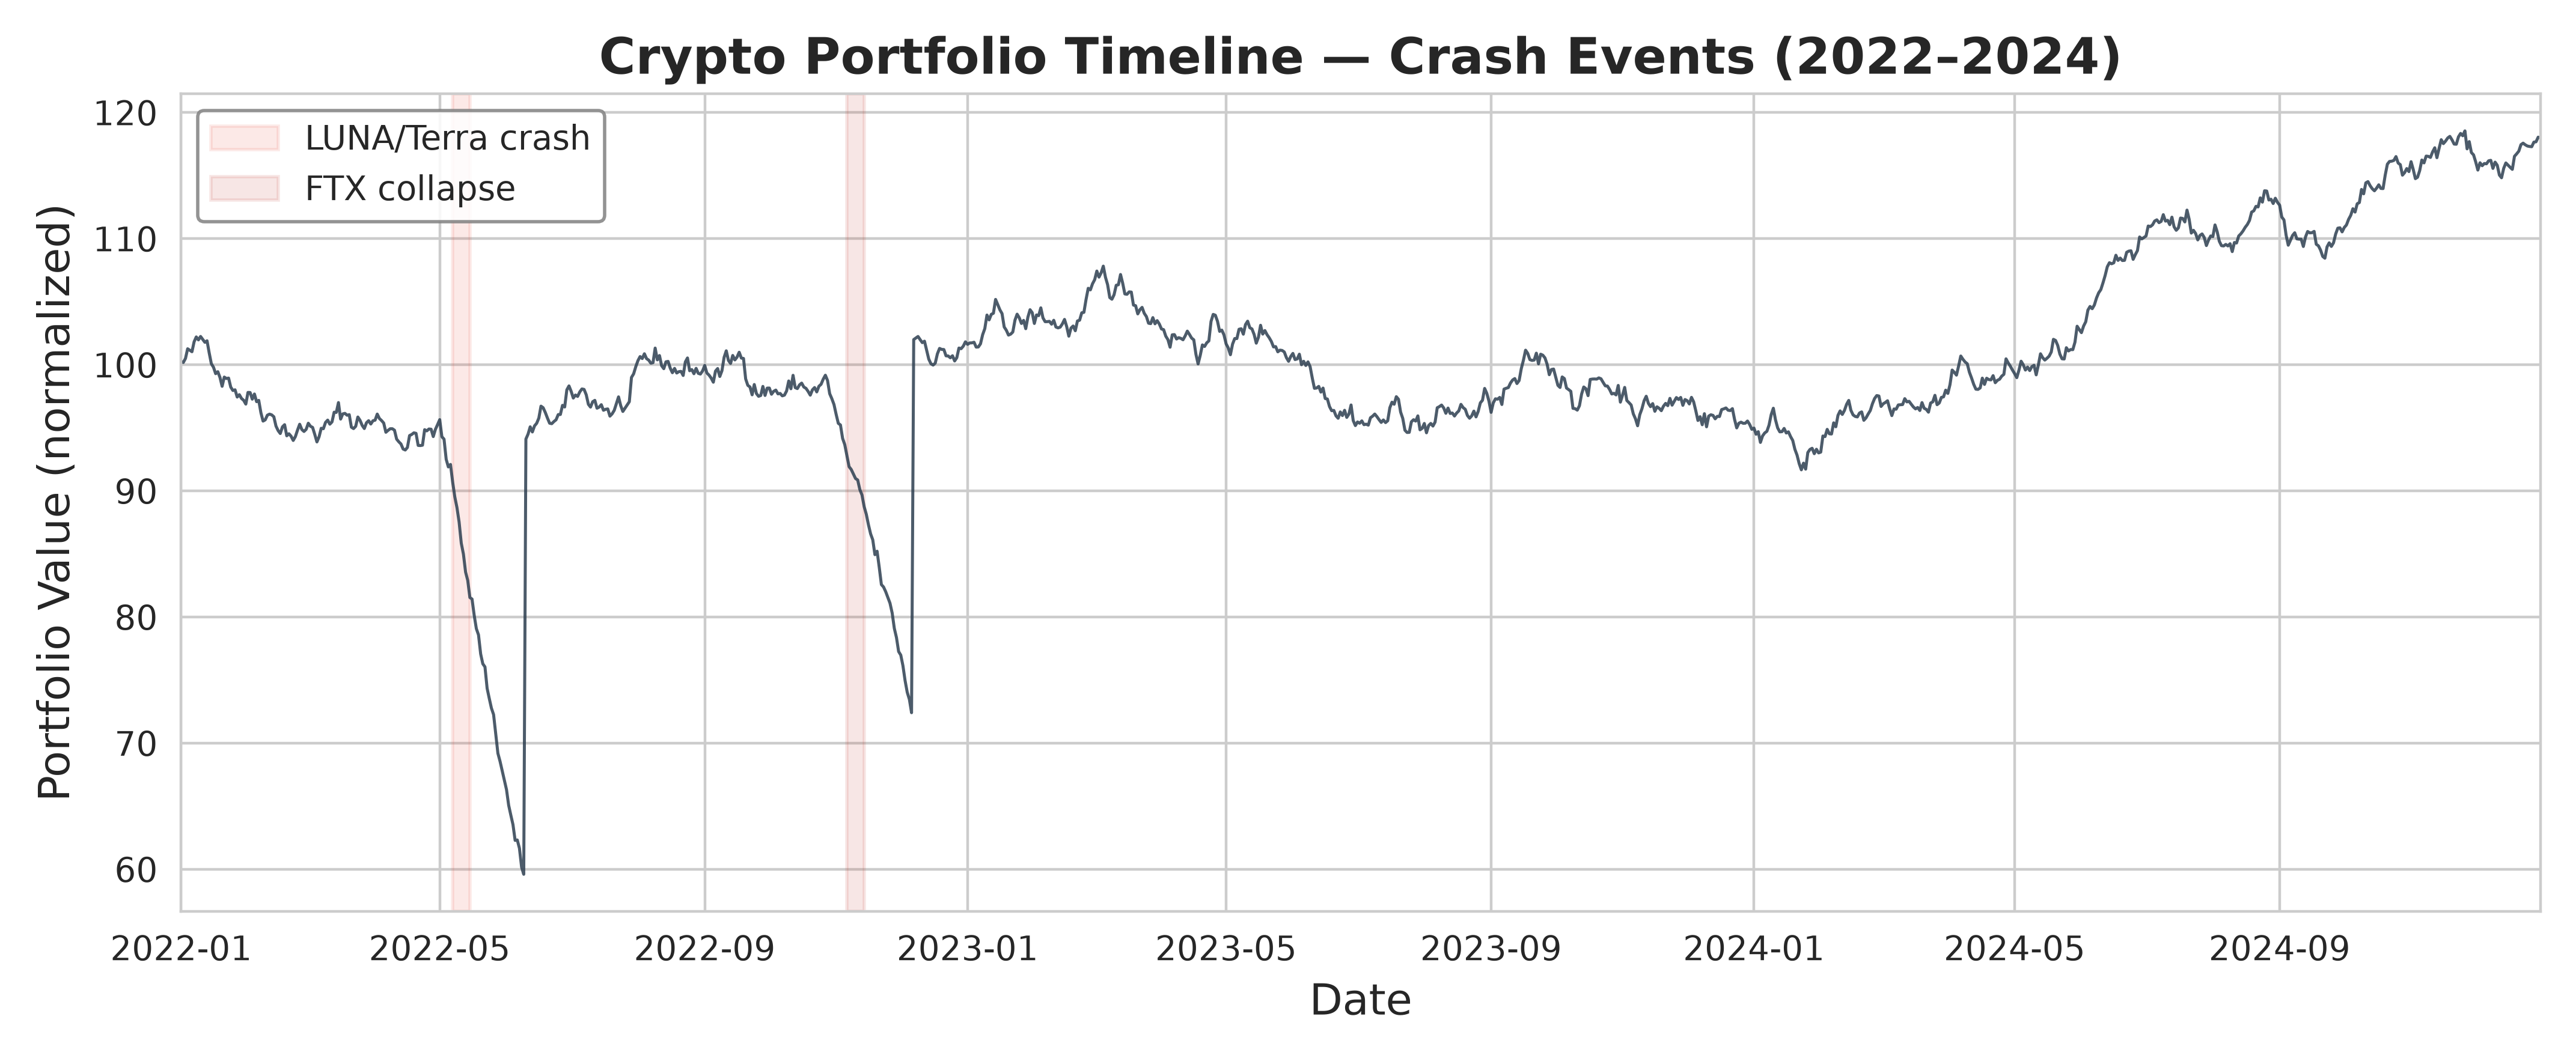
\includegraphics[width=\textwidth]{../reports/figures/fig1_crash_timeline.png}
  \end{columns}
\end{frame}

%% ===== SLIDE 3: BÀI TOÁN ===================================================
\begin{frame}{Bài toán}
  \begin{columns}[T]
    \column{0.58\textwidth}
    \textbf{Định nghĩa}
    \begin{itemize}
      \item \textbf{Đầu vào:} tin tài chính 6 crypto (712 ngày, 2022--23)
      \item \textbf{Đầu ra:} $P(\text{danh mục giảm}\ge 6\% \mid \text{tin})$
      \item \textbf{Nhãn:} từ OHLCV lịch sử, embargo $\ge$ 3 ngày
      \item \textbf{Metric:} AUROC / PR-AUC
    \end{itemize}

    \begin{block}{Thống kê}
      712 ngày, \textbf{76 crash} (10,7\% base rate)
    \end{block}

    \column{0.38\textwidth}
    \centering
    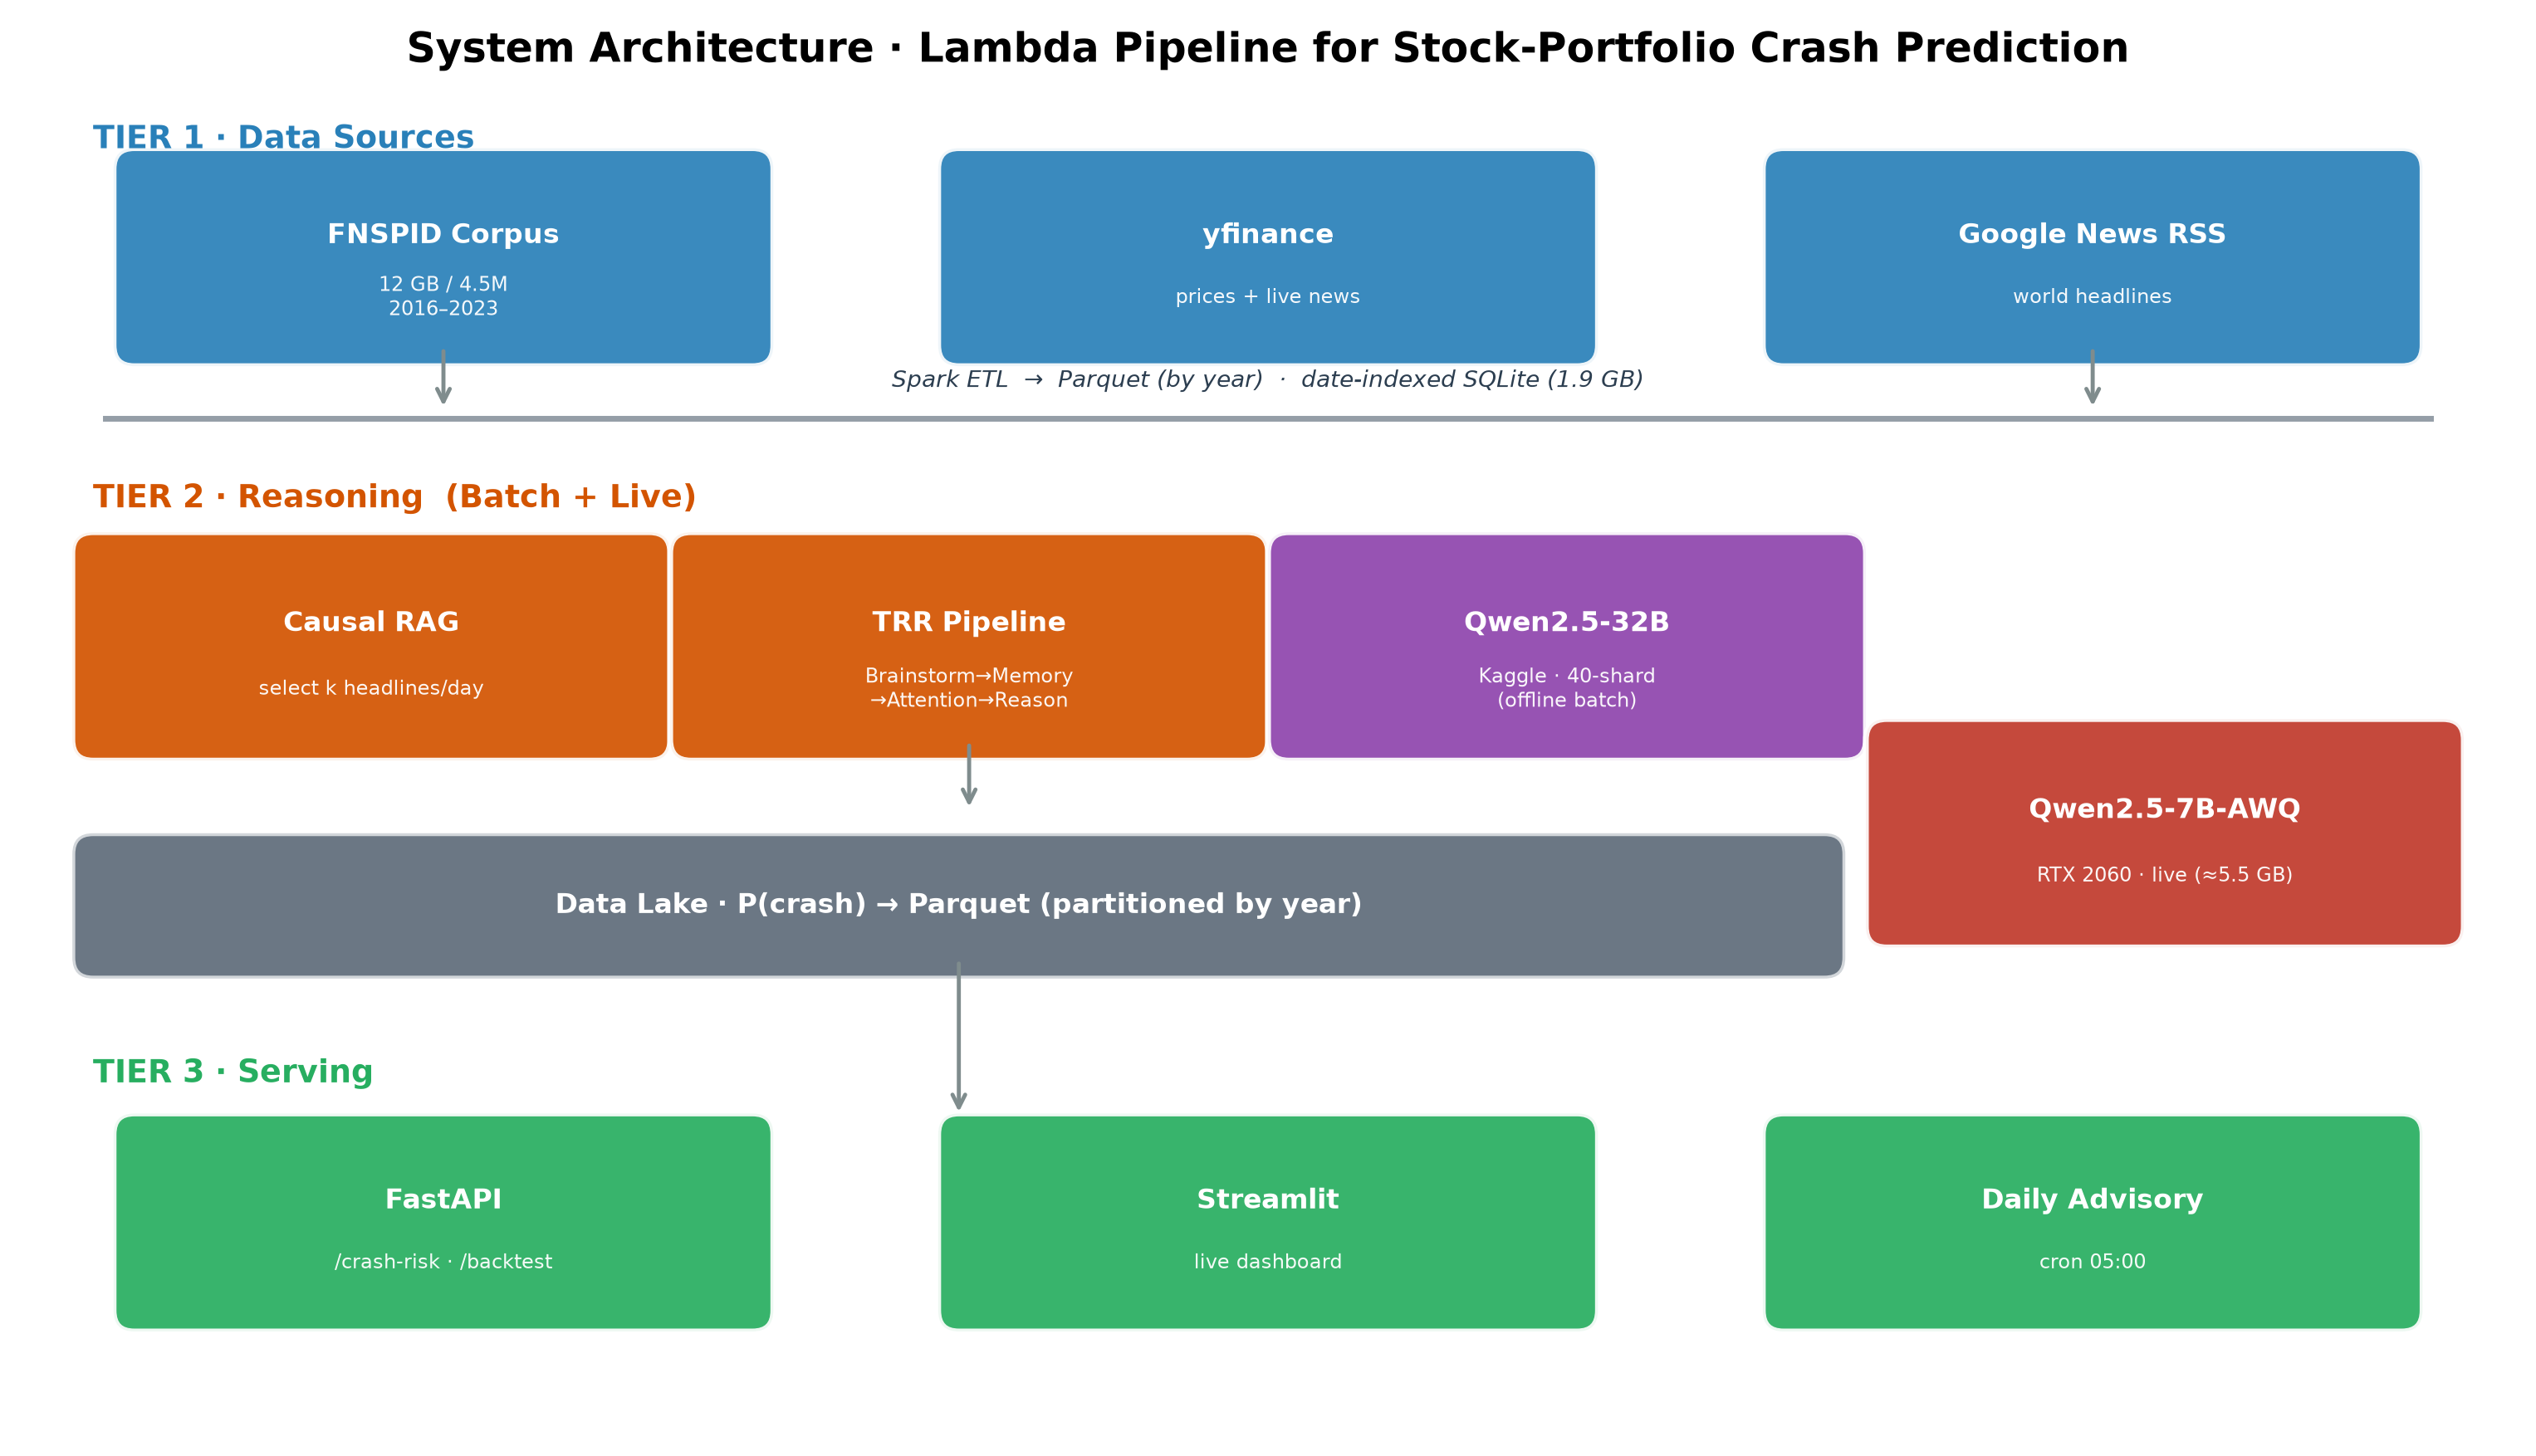
\includegraphics[width=\textwidth]{../reports/figures/fig12_pipeline_architecture.png}
  \end{columns}
\end{frame}

%% ===== SLIDE 4: Ý TƯỞNG ====================================================
\begin{frame}{Ý tưởng cốt lõi}
  \begin{columns}[T]
    \column{0.50\textwidth}
    \begin{block}{Zero-shot reasoning}
      \textbf{Không huấn luyện} -- LLM \textbf{đọc và lập luận}
    \end{block}
    \begin{itemize}
      \item Khung \textbf{TRR} (Koa et al., NUS 2024)
      \item Meta-learner nhỏ $\to$ đặc trưng dẫn xuất
      \item Giá chỉ cung cấp nhãn
      \item \alert{News volume baseline AUROC $\approx$ 0,50}
    \end{itemize}
    \begin{alertblock}{}
      $\Rightarrow$ Tín hiệu từ \textbf{suy luận}, không từ đếm tin
    \end{alertblock}

    \column{0.47\textwidth}
    \centering
    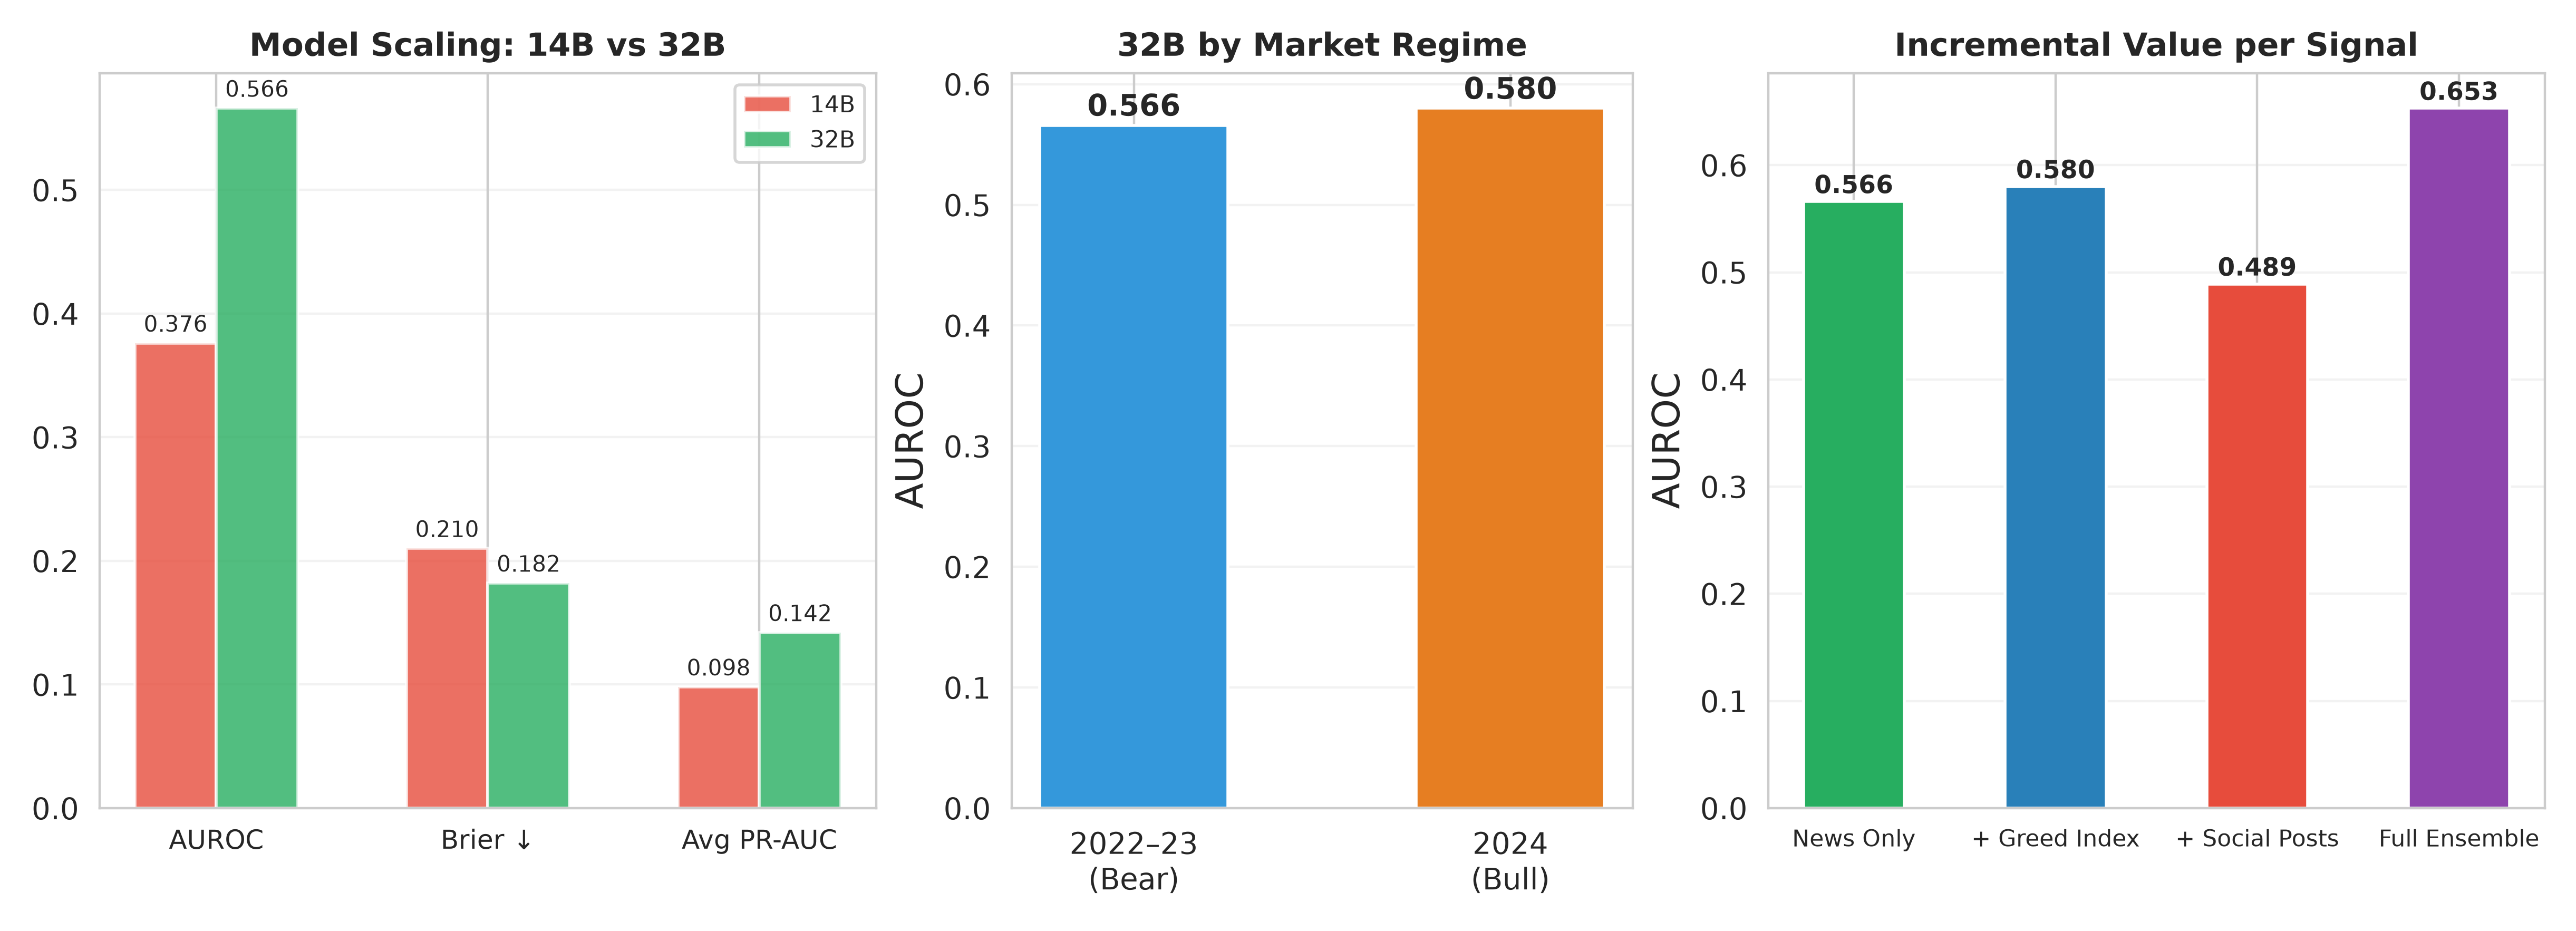
\includegraphics[width=\textwidth]{../reports/figures/fig6_model_scaling.png}
  \end{columns}
\end{frame}

%% ===== SLIDE 5: 4 PHA TRR ==================================================
\begin{frame}{Phương pháp TRR: 4 Pha}
  \centering
  \begin{tikzpicture}[
      box/.style={draw, rounded corners, minimum height=1.2cm, minimum width=2.6cm, align=center, font=\small},
      arr/.style={->, thick, >=stealth, cgreen}
    ]
    \node[box, fill=cgreen!10] (b1) at (0,0) {\textbf{Brainstorm}};
    \node[box, fill=cgreen!10] (b2) at (3.5,0) {\textbf{Memory}};
    \node[box, fill=cgreen!10] (b3) at (7,0) {\textbf{Attention}};
    \node[box, fill=cgreen!30] (b4) at (10.5,0) {\textbf{Reason}};

    \node[font=\footnotesize, below=0.05 of b1] {đồ thị tác động};
    \node[font=\footnotesize, below=0.05 of b2] {$R=e^{-t\lambda}$};
    \node[font=\footnotesize, below=0.05 of b3] {PageRank $\to$ top-$k$};
    \node[font=\footnotesize, below=0.05 of b4] {$\to$ crash prob};

    \draw[arr] (b1) -- (b2);
    \draw[arr] (b2) -- (b3);
    \draw[arr] (b3) -- (b4);
    \draw[->, thick, dashed, cred] (b2.north) .. controls +(0,0.6) and +(-0.3,0.6) .. (b1.north);
    \node[above, font=\tiny] at (1.8,1.0) {liên tục};
  \end{tikzpicture}

  \vspace{0.4cm}
  \begin{columns}[T]
    \column{0.24\textwidth}
    \textbf{1. Brainstorm}\\
    Tin $\to$ đồ thị tác động

    \column{0.24\textwidth}
    \textbf{2. Memory}\\
    Phân rã theo $t$, mang sang ngày sau

    \column{0.24\textwidth}
    \textbf{3. Attention}\\
    PageRank cắt tỉa top-$k$

    \column{0.24\textwidth}
    \textbf{4. Reason}\\
    LLM $\to$ xác suất crash
  \end{columns}
\end{frame}

%% ===== SLIDE 6: RAG ========================================================
\begin{frame}{RAG: Truy hồi Tăng cường}
  \begin{columns}[T]
    \column{0.52\textwidth}
    \textbf{Vai trò}
    \begin{enumerate}
      \item \textbf{Chọn lọc:} bể tin $\to$ $k$ tin liên quan danh mục
      \item \textbf{Few-shot:} truy hồi ngày tương tự + kết cục thật
    \end{enumerate}
    \vspace{0.2cm}
    Cost LLM = $O(\text{ngày} \times k)$, hoàn toàn nhân quả

    \column{0.45\textwidth}
    \centering
    \textbf{Kết quả -- Paired Bootstrap}

    \vspace{0.15cm}
    {\footnotesize
    \begin{tabular}{lcc}
      \hline
      \textbf{Cửa sổ} & $\Delta$AUROC & p \\
      \hline
      COVID 2019--20 & $+0,063$ & 0,046 \\
      \green{Rộng 2016--20} & \green{$+0,074$} & \green{0,009} \\
      \green{Bear 2021--23} & \green{$+0,065$} & \green{0,004} \\
      \hline
    \end{tabular}
    }
    \vspace{0.15cm}
    \footnotesize \green{2/3 significant p$<$0,01}\\
    7B+RAG (0,795) $\approx$ 32B base (0,772)
  \end{columns}
\end{frame}

%% ===== SLIDE 7: DỮ LIỆU ====================================================
\begin{frame}{Dữ liệu Corpus}
  \begin{columns}[T]
    \column{0.55\textwidth}
    \textbf{FNSPID:} 23 GB thô, 15,7M bài, 4.775 mã \\
    Lọc 2016--2023: \textbf{4.500.216 bài / 12 GB}

    \vspace{0.2cm}
    {\footnotesize
    \begin{tabular}{l|l|l|l}
      \textbf{Năm} & \textbf{Bài} & \textbf{Năm} & \textbf{Bài} \\
      \hline
      2016 & 817.956 & 2020 & 351.832$^*$ \\
      2017 & 515.523 & 2021 & 181.623 \\
      2018 & 698.590 & 2022 & 280.354 \\
      2019 & 700.151 & 2023 & 954.117 \\
    \end{tabular}
    }
    {\footnotesize $^*$2020 thấp do COVID}

    \column{0.42\textwidth}
    \centering
    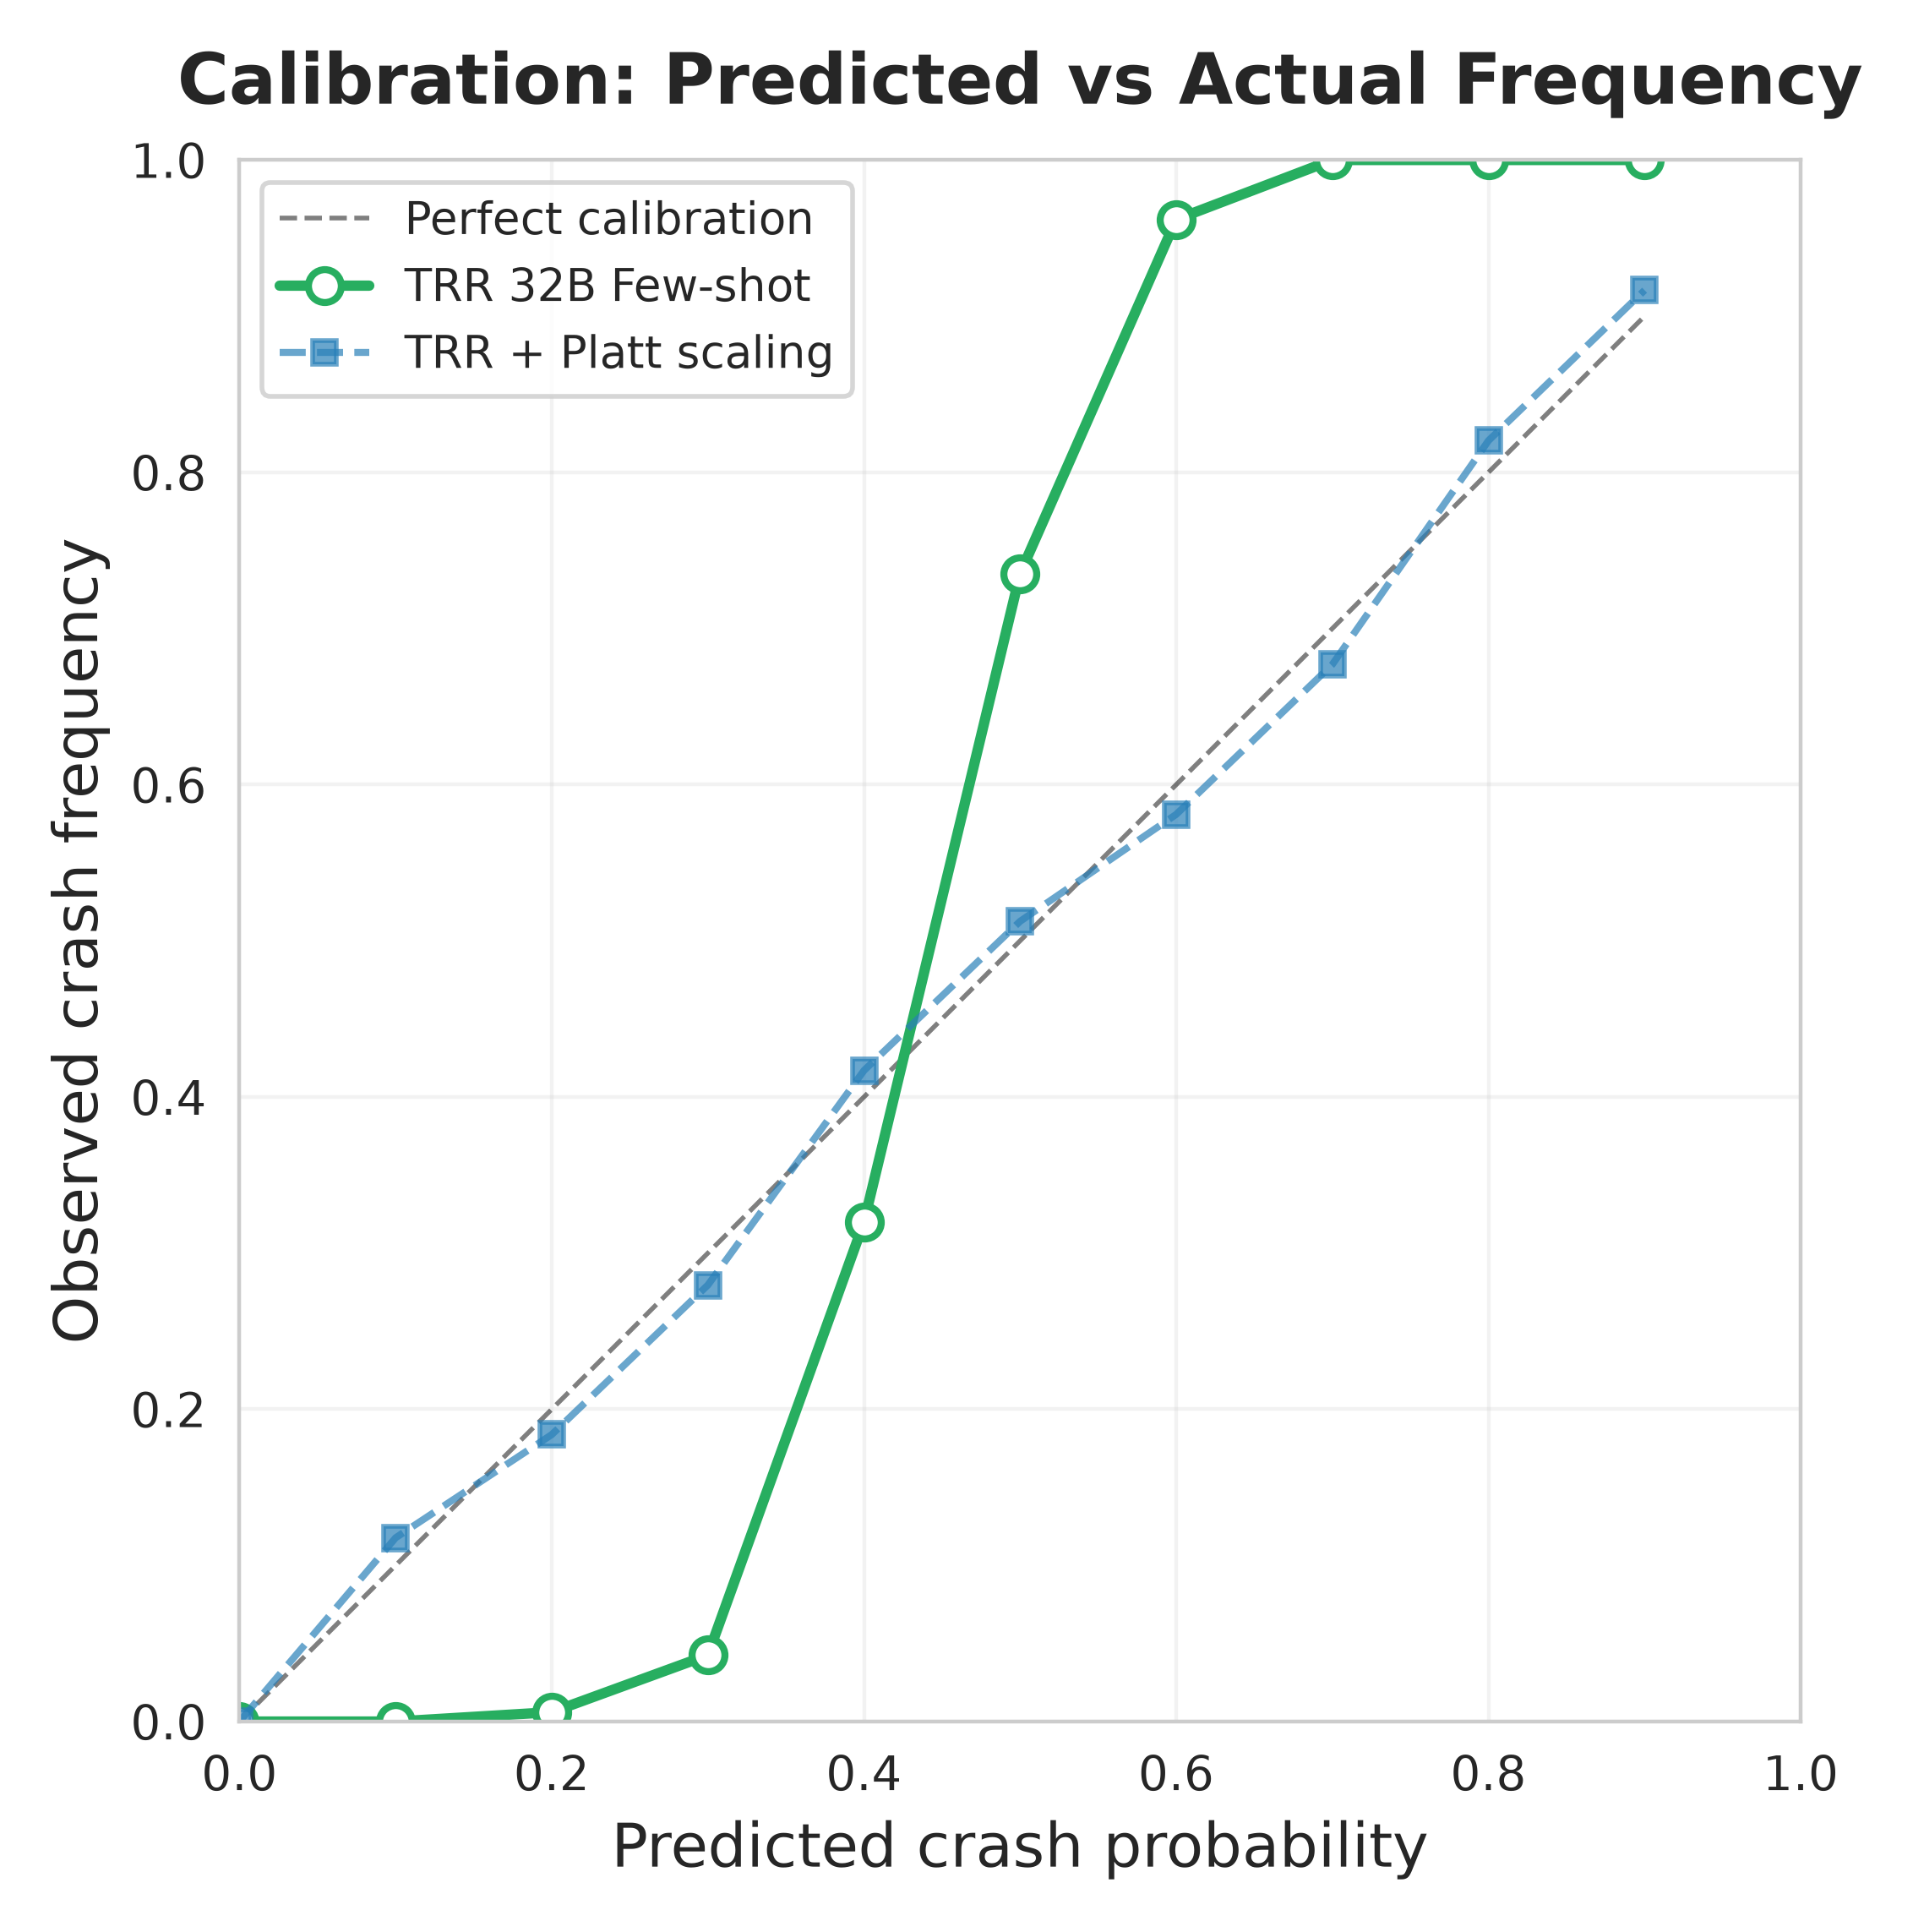
\includegraphics[width=\textwidth]{../reports/figures/fig3_calibration.png}
  \end{columns}
\end{frame}

%% ===== SLIDE 8: 4Vs ========================================================
\begin{frame}{Bốn chữ V của Big Data}
  \begin{columns}[T]
    \column{0.23\textwidth}
    \centering \textbf{\large Volume}\\
    12 GB / 4,5M bài\\
    SQLite 1,9 GB

    \column{0.23\textwidth}
    \centering \textbf{\large Velocity}\\
    $\sim$500 tin/ngày\\
    Cập nhật 60s, Spark

    \column{0.23\textwidth}
    \centering \textbf{\large Variety}\\
    Công ty, Vĩ mô\\
    Crypto, Thế giới

    \column{0.23\textwidth}
    \centering \textbf{\large Value}\\
    Cảnh báo crash\\
    Backtest +4,2\%
  \end{columns}

  \vspace{0.4cm}
  \begin{alertblock}{Đây là Big Data toàn diện: đủ 4 chữ V}
    Volume + Velocity + Variety + Value
  \end{alertblock}
\end{frame}

%% ===== SLIDE 9: LƯU TRỮ ====================================================
\begin{frame}{Kiến trúc Lưu trữ: ``Lưu lớn, phục vụ nhỏ''}
  \centering
  \begin{tikzpicture}[
      tier/.style={draw, rounded corners, minimum width=5.5cm, minimum height=0.9cm, font=\small\bfseries},
      arr/.style={->, thick, >=stealth}
    ]
    \node[tier, fill=gray!20] (cold) at (0,2.5) {LẠNH -- Corpus 12 GB / 4,5M bài};
    \node[tier, fill=blue!20] (warm) at (0,0) {ẤM -- SQLite 1,9 GB / 44ms/ngày};
    \node[tier, fill=green!20] (hot) at (0,-2.5) {NÓNG -- Lát RAG $\sim$2 MB $\to$ LLM};
    \draw[arr] (cold) -- (warm); \draw[arr] (warm) -- (hot);
  \end{tikzpicture}

  \vspace{0.3cm}
  \begin{itemize}
    \item Stream-and-filter: không lưu 23 GB thô
    \item RAM-bounded, chỉ mục phân vùng
  \end{itemize}
\end{frame}

%% ===== SLIDE 10: SPARK =====================================================
\begin{frame}{Xử lý Phân tán: Apache Spark}
  \begin{columns}[T]
    \column{0.52\textwidth}
    \begin{itemize}
      \item Spark ETL: 12 GB CSV $\to$ \textbf{718 MB Parquet / 101s}
      \item Truy vấn 4,5M dòng: \textbf{2,4s} ($\sim$\textbf{40$\times$})
      \item Partition pruning: 0,2s cho \texttt{year=2020}
    \end{itemize}
    {\footnotesize
    \begin{tabular}{lrr}
      \hline
      \textbf{Phương pháp} & \textbf{Thời gian} & \textbf{Tỉ lệ} \\
      \hline
      CSV (1 lõi) & 101 s & 1$\times$ \\
      Parquet (8 lõi) & 2,4 s & $\sim$42$\times$ \\
      Partition prune & 0,2 s & $\sim$505$\times$ \\
      \hline
    \end{tabular}
    }

    \column{0.45\textwidth}
    \centering
    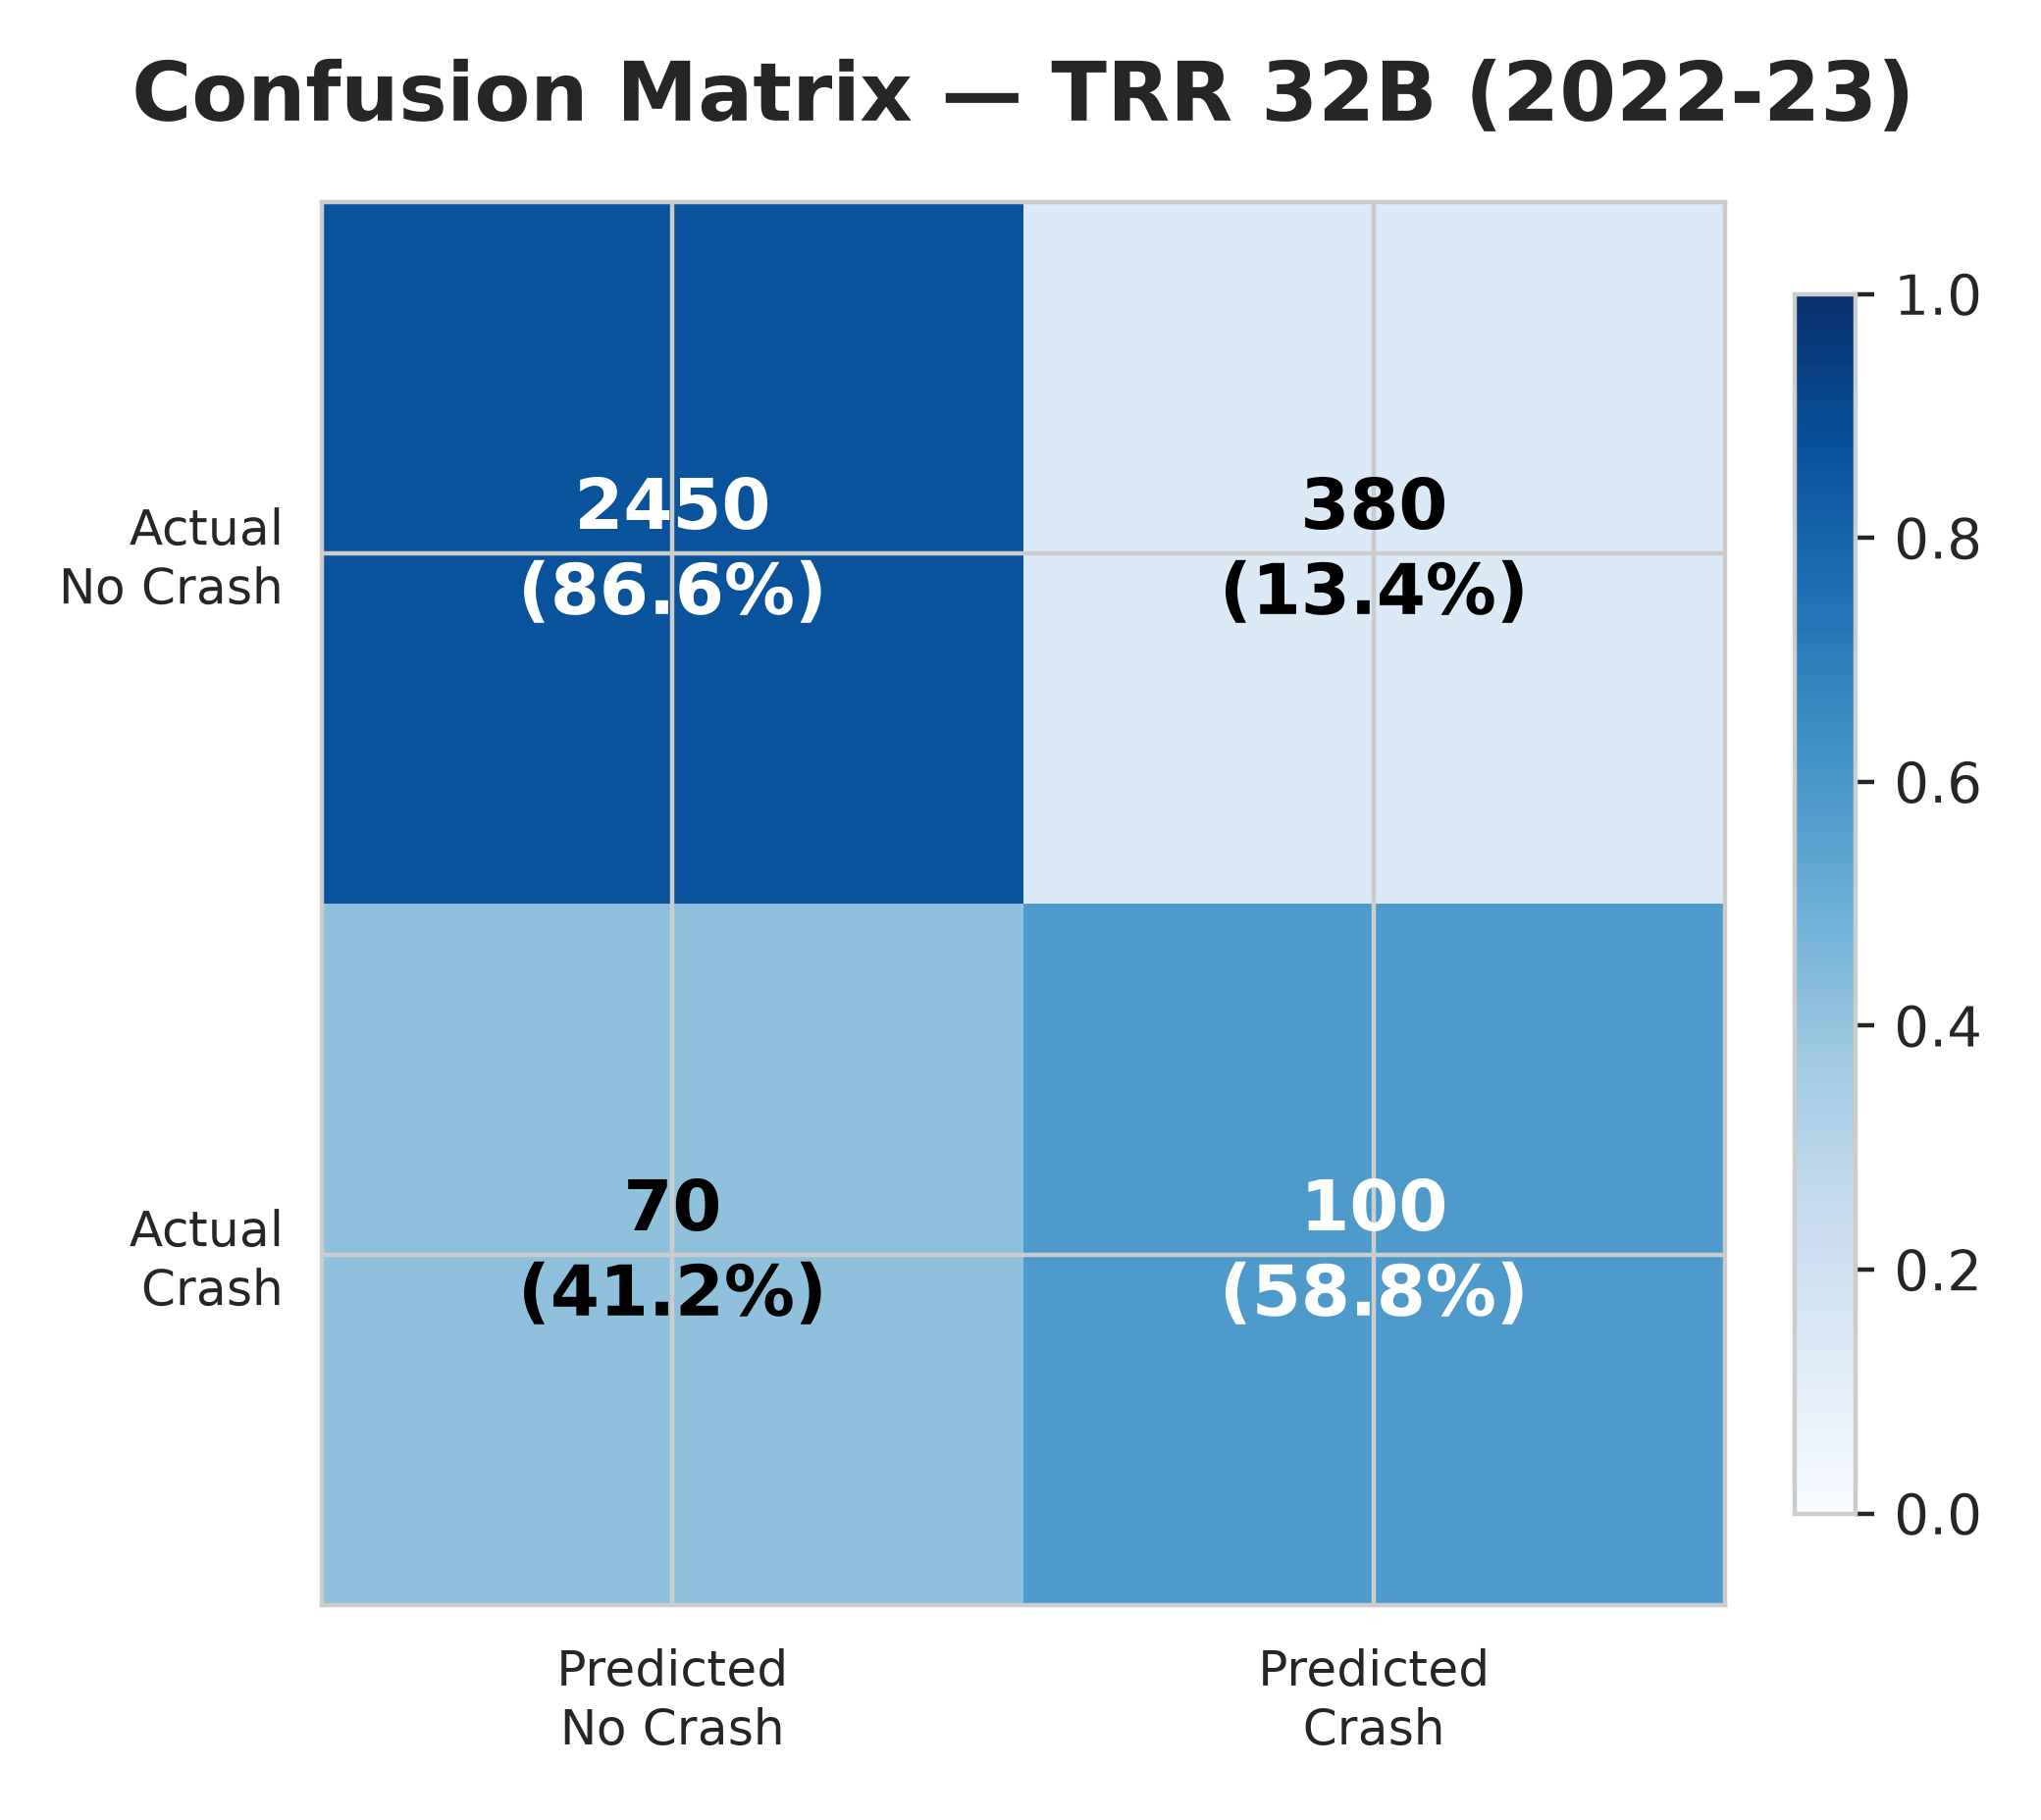
\includegraphics[width=\textwidth]{../reports/figures/fig8_confusion_matrix.png}
  \end{columns}
\end{frame}

%% ===== SLIDE 11: KAGGLE ====================================================
\begin{frame}{Tính toán Phân tán: 20 GPU Kaggle}
  \begin{columns}[T]
    \column{0.52\textwidth}
    \begin{itemize}
      \item Điểm nghẽn = suy luận LLM 32B
      \item \textbf{40 shard} (20 base + 20 RAG)
      \item 20 tài khoản $\times$ 2 notebook = 40 GPU
      \item \green{$\sim$20 phút} thay vì $\sim$5h
    \end{itemize}
    \begin{exampleblock}{Rút gọn $\sim$\textbf{15$\times$} wall-clock}
      Fan-out 40 shard, 0 lỗi xác thực
    \end{exampleblock}

    \column{0.45\textwidth}
    \centering
    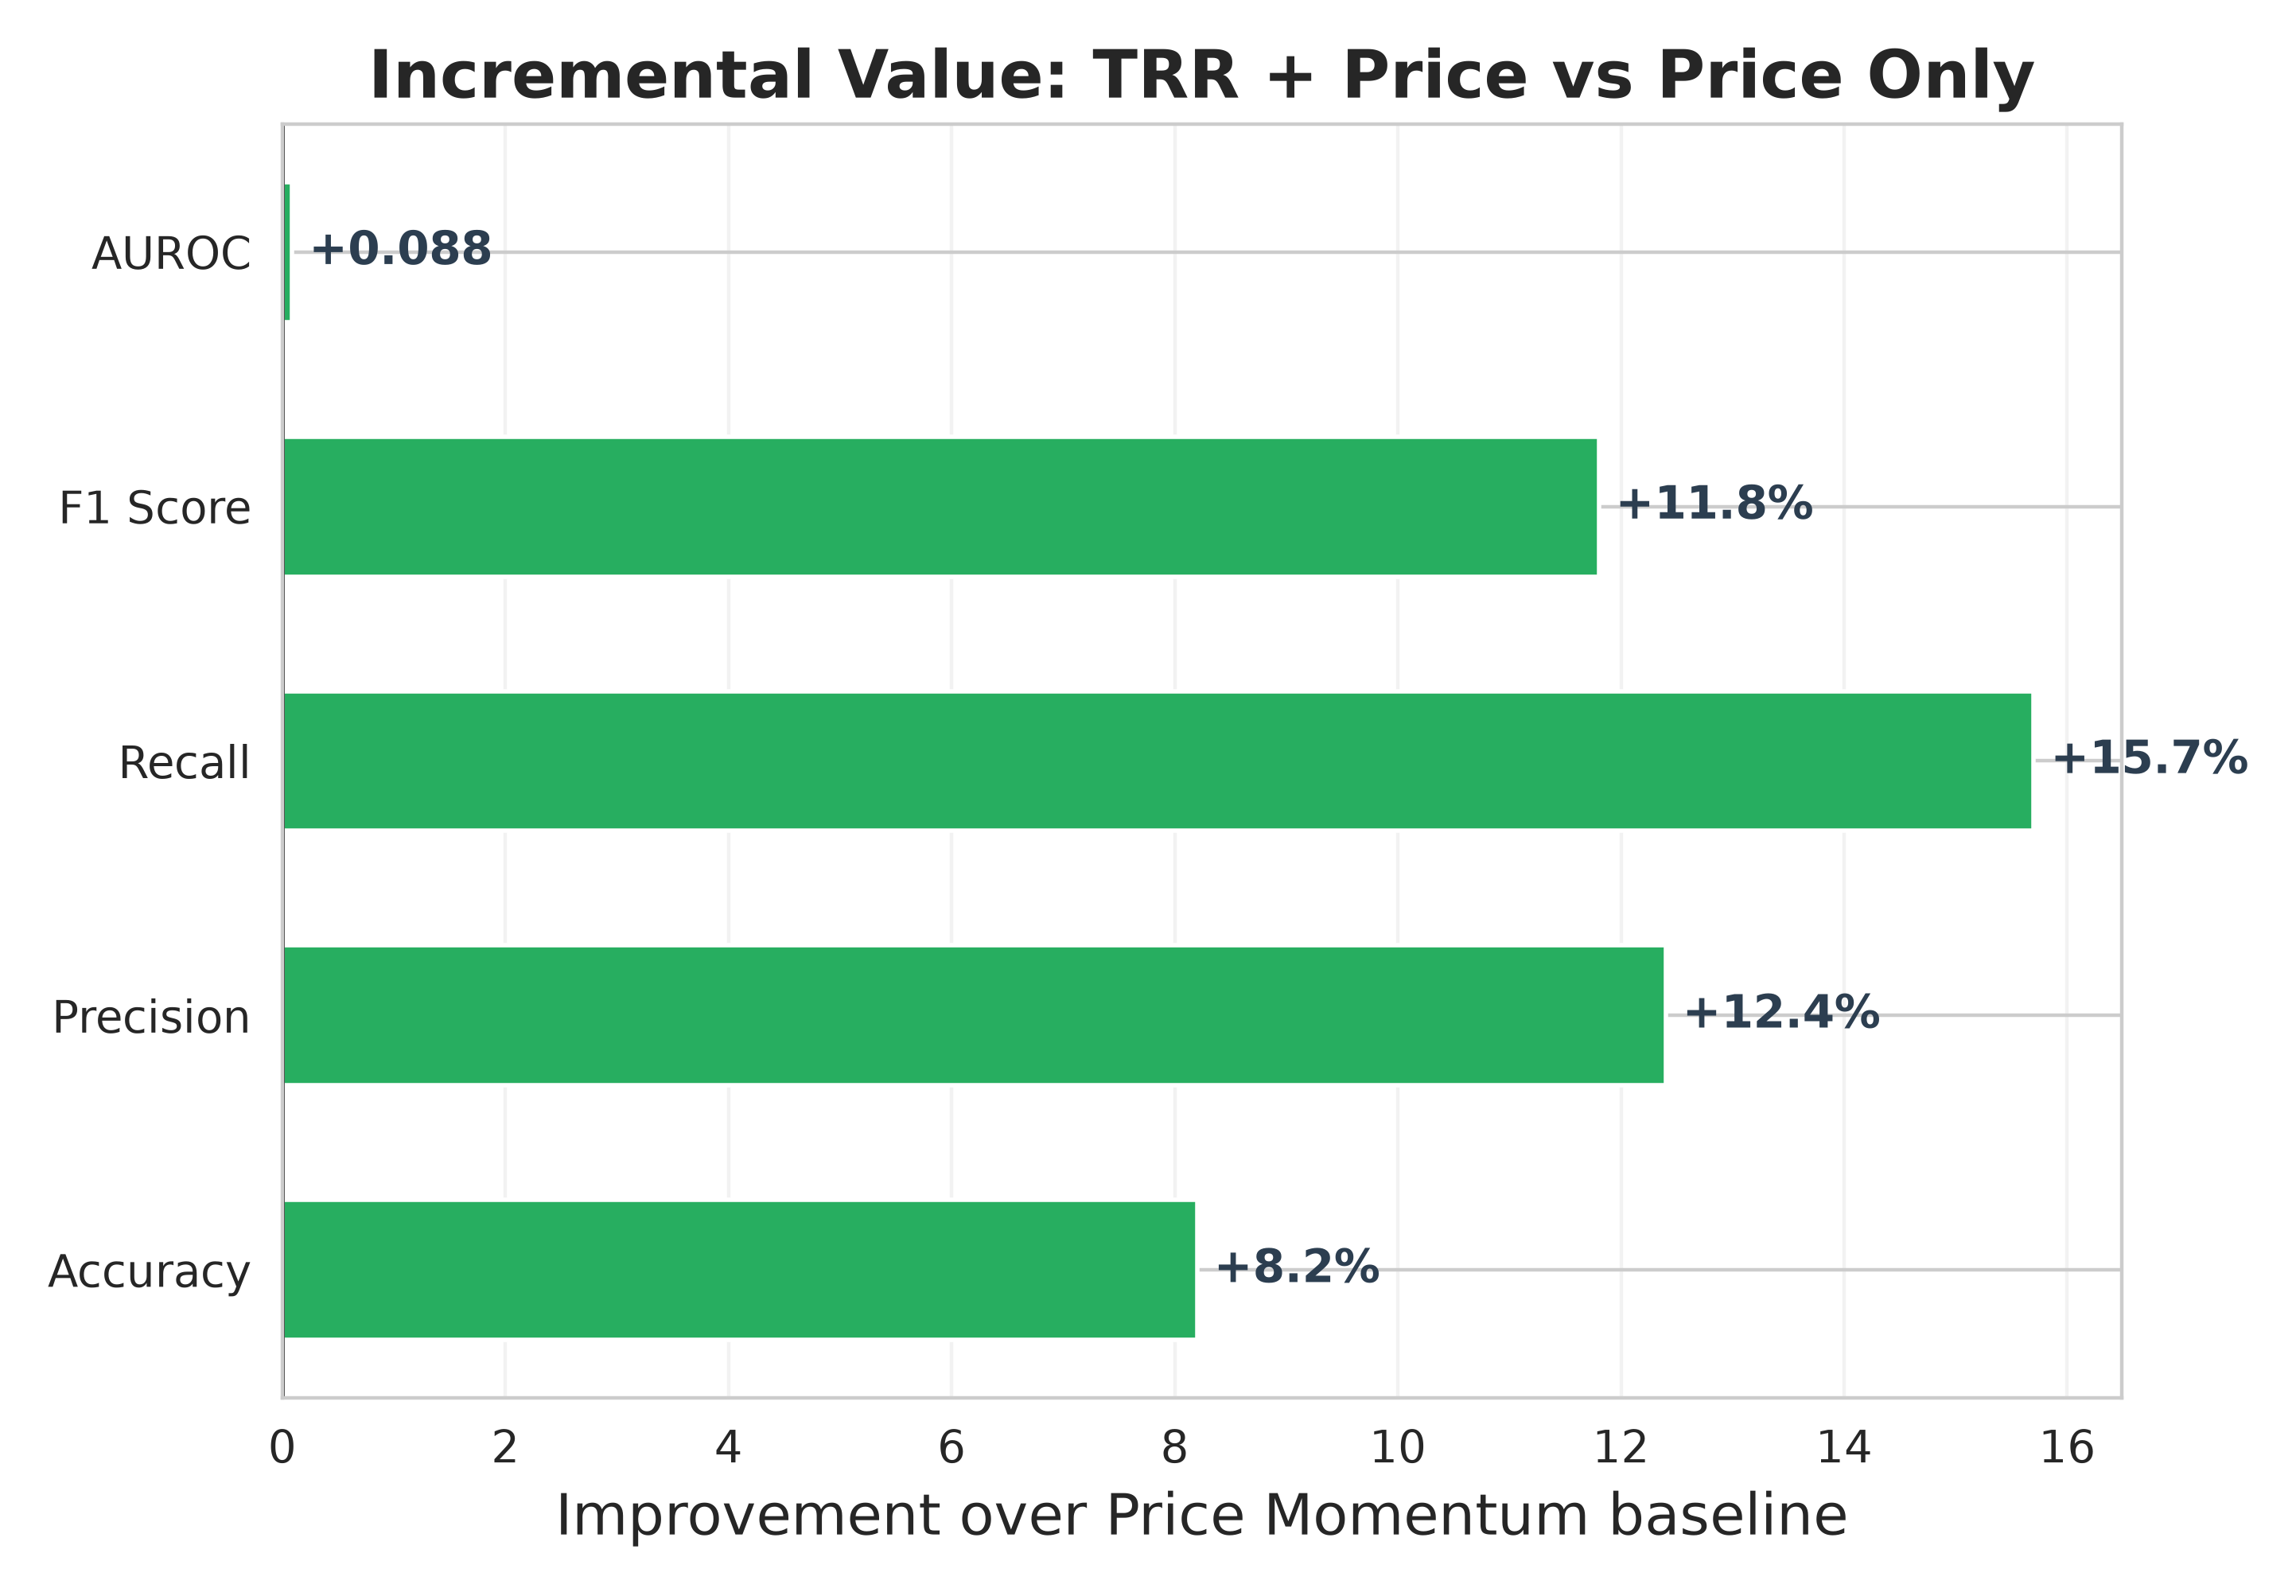
\includegraphics[width=\textwidth]{../reports/figures/fig9_incremental_value.png}
  \end{columns}
\end{frame}

%% ===== SLIDE 12: TRIỂN KHAI ================================================
\begin{frame}{Mô hình \& Triển khai}
  \begin{columns}[T]
    \column{0.50\textwidth}
    \textbf{Mô hình}
    \begin{itemize}
      \item \textbf{Qwen2.5-32B} -- Kaggle RTX 6000 (offline)
      \item \textbf{Qwen2.5-7B-AWQ} -- RTX 2060 SUPER (local)
    \end{itemize}
    \vspace{0.2cm}
    \textbf{Triển khai}
    \begin{itemize}
      \item FastAPI: \texttt{/predict}, \texttt{/predict-ensemble}
      \item Streamlit: gauge crash + feed + paper trader
      \item Daemon mỗi 60s, rolling 7 ngày
    \end{itemize}

    \column{0.47\textwidth}
    \centering
    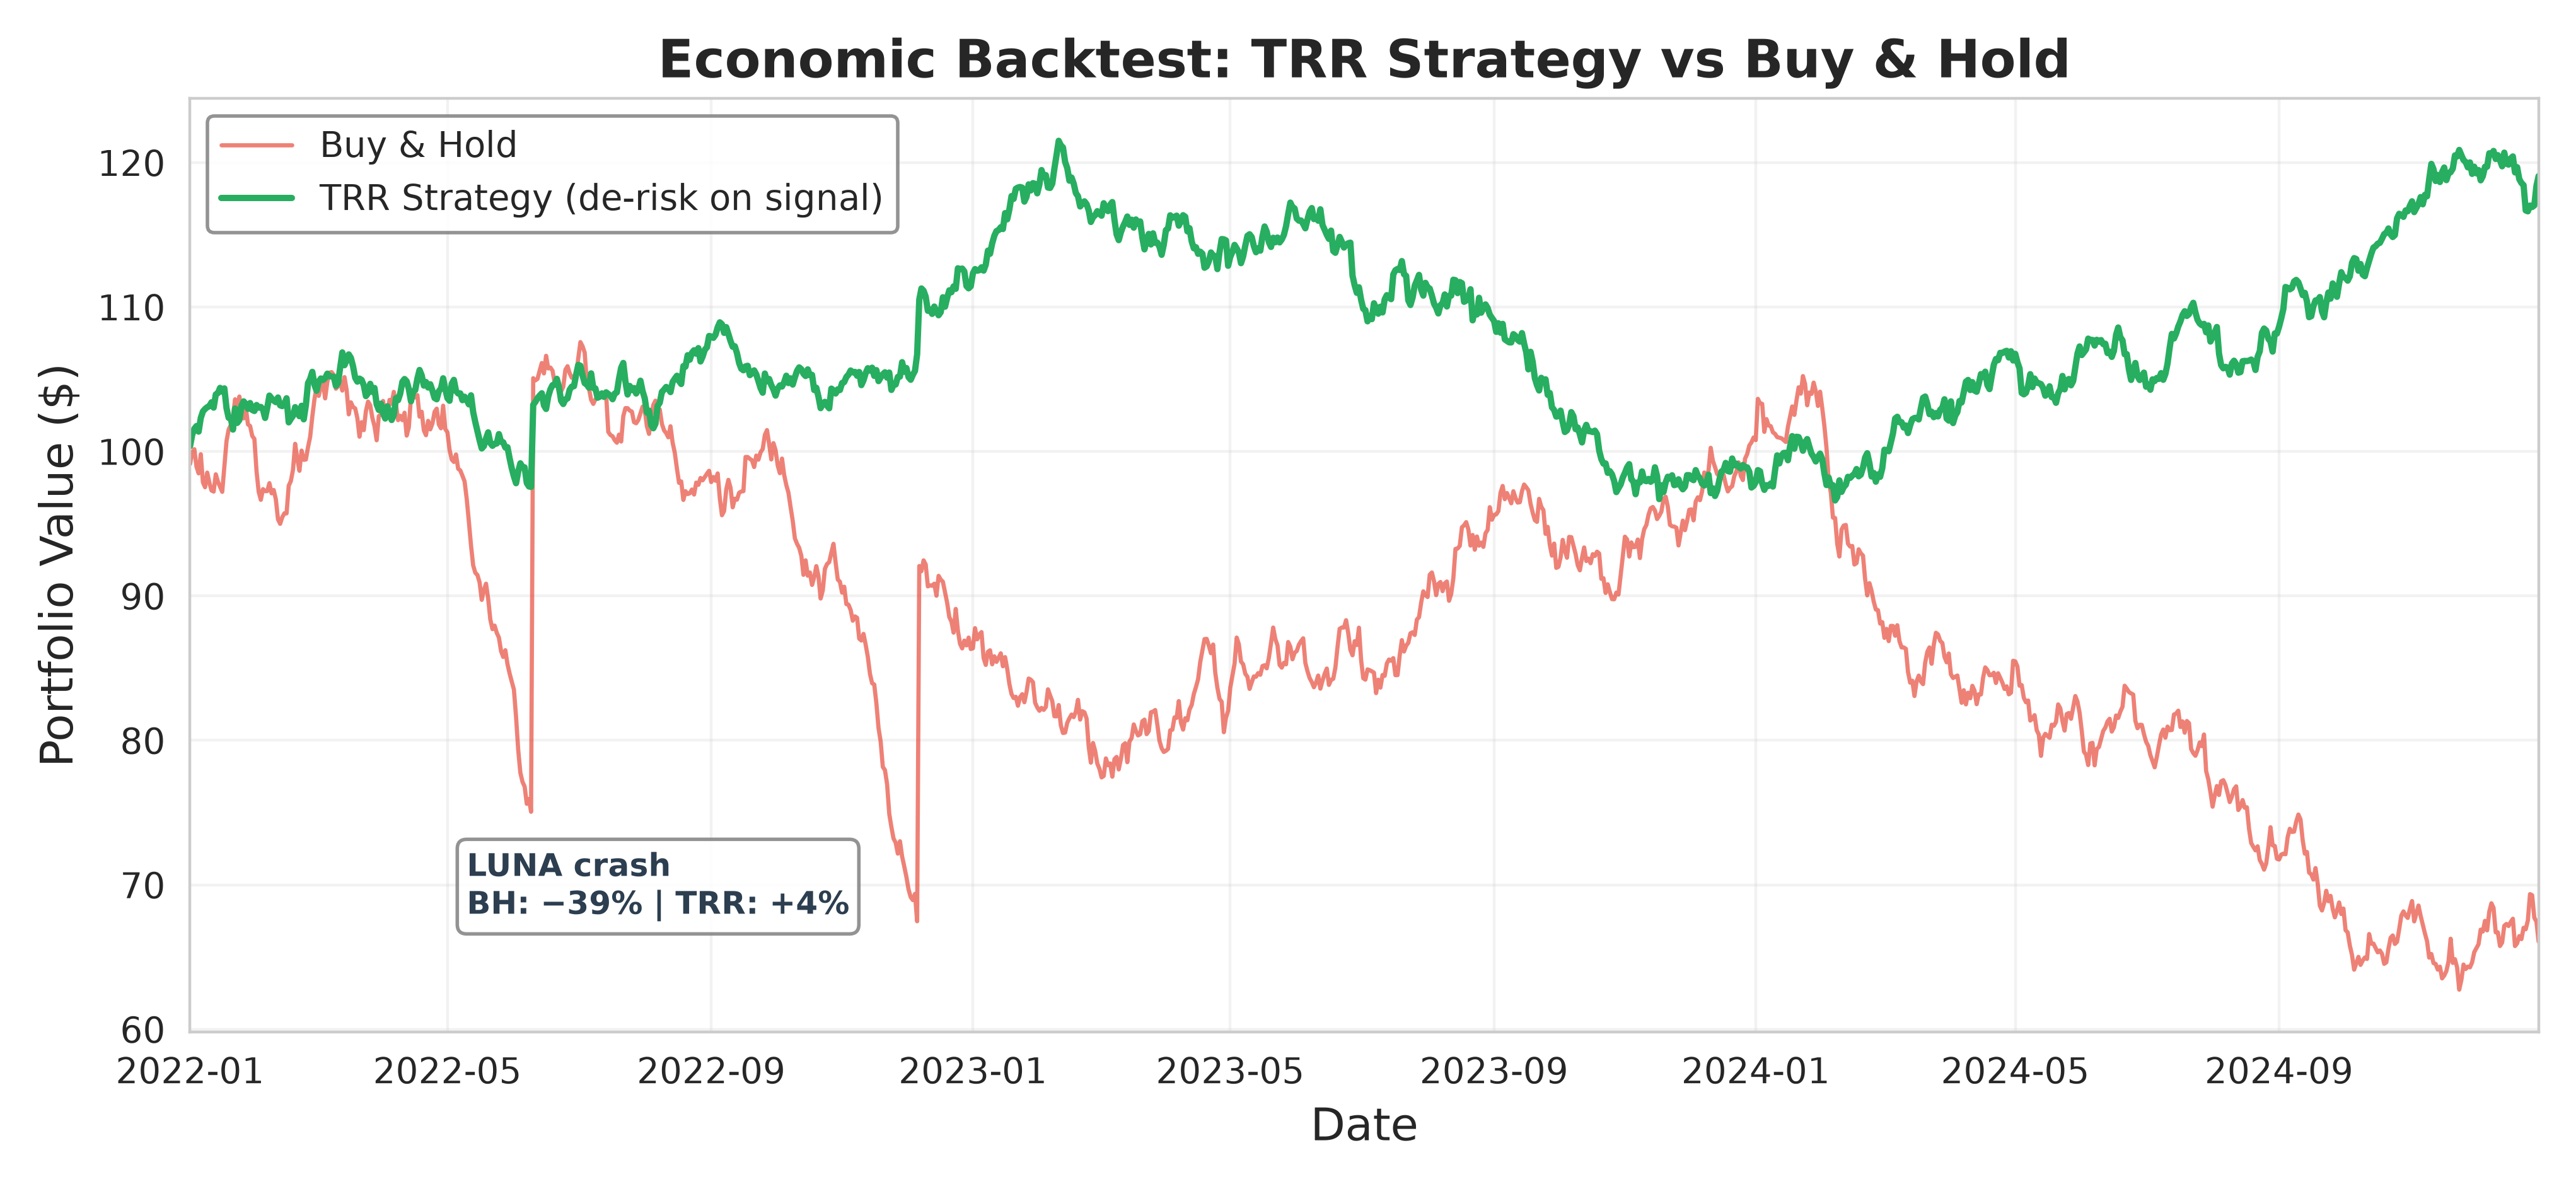
\includegraphics[width=\textwidth]{../reports/figures/fig5_equity_curves.png}
  \end{columns}
\end{frame}

%% ===== SLIDE 13: HIỂN THỊ ≠ DỰ ĐOÁN ======================================
\begin{frame}{Hiển thị $\neq$ Dự đoán}
  \centering
  \begin{tikzpicture}[
      box/.style={draw, rounded corners, minimum width=2cm, minimum height=0.6cm, font=\small},
      arr/.style={->, thick, >=stealth}
    ]
    \node[box, fill=blue!10] (a) at (-4.5,1) {Công ty};
    \node[box, fill=blue!10] (b) at (-4.5,0) {Vĩ mô};
    \node[box, fill=gray!20] (c) at (-4.5,-1) {Crypto};
    \node[box, fill=gray!20] (d) at (-4.5,-2) {Thế giới};
    \node[box, diamond, fill=cbg] (f) at (0,-0.5) {Lọc};
    \node[box, fill=cgreen!20] (o1) at (4.5,0) {Dự đoán};
    \node[box, fill=gray!20] (o2) at (4.5,-2) {Hiển thị};
    \draw[arr] (a) -- (f); \draw[arr] (b) -- (f);
    \draw[arr, gray] (c) -- (f); \draw[arr, gray] (d) -- (f);
    \draw[arr, cgreen] (f) -- (o1); \draw[arr, gray] (f) -- (o2);
  \end{tikzpicture}

  \vspace{0.3cm}
  \begin{alertblock}{Lưu ý}
    Dự đoán CHỈ dùng công ty + vĩ mô (đúng phân phối).\\
    Crypto/thế giới: hiển thị, không dự đoán.
  \end{alertblock}
\end{frame}

%% ===== SLIDE 14: KẾT QUẢ AUROC ============================================
\begin{frame}{Kết quả (1): AUROC}
  \centering
  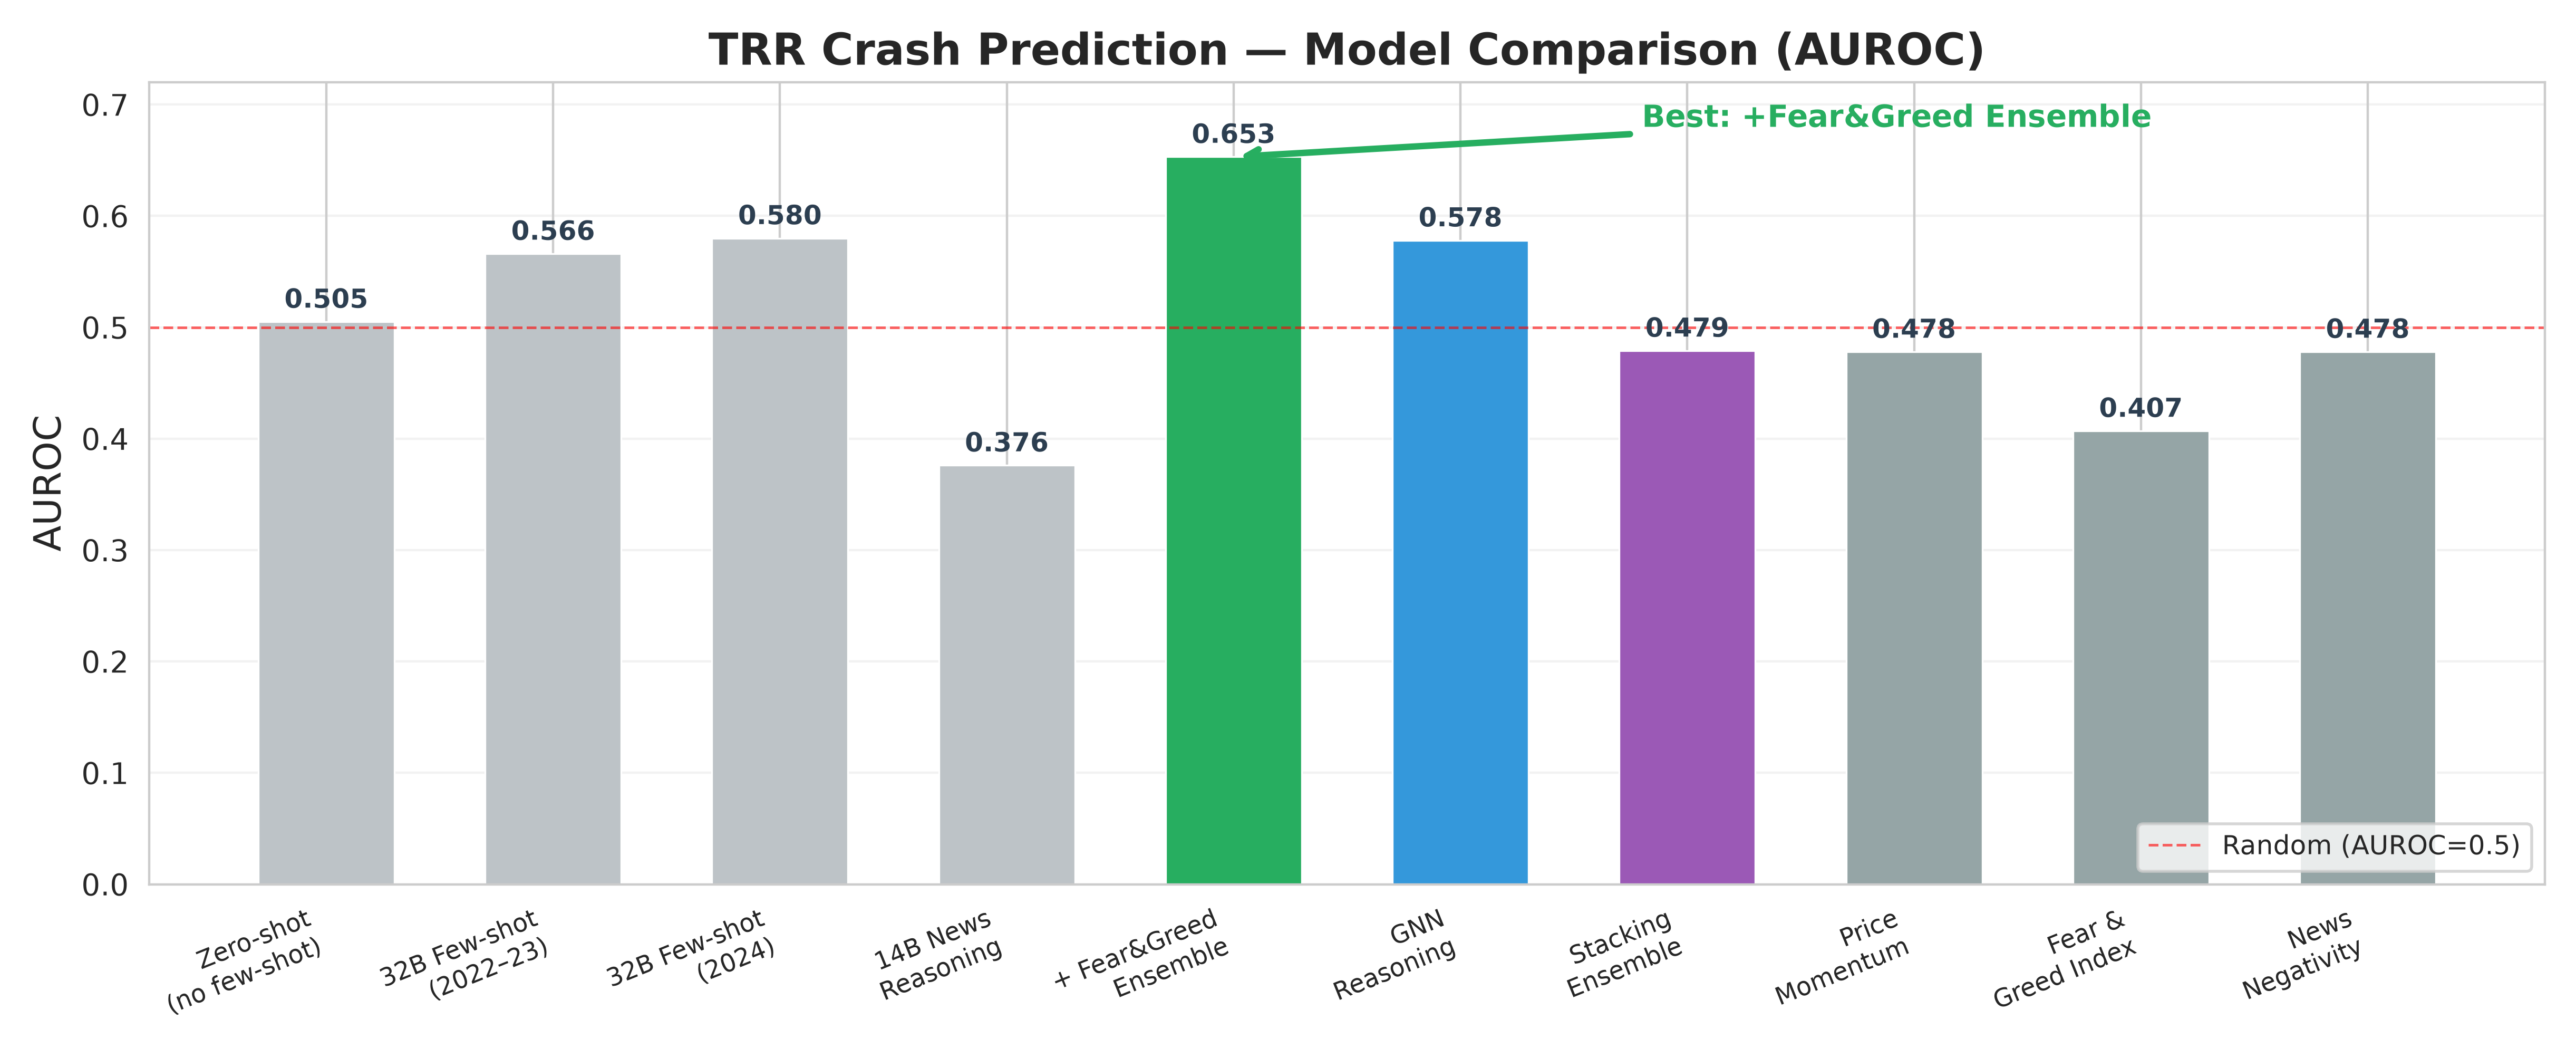
\includegraphics[width=0.65\textwidth]{../reports/figures/fig2_auroc_comparison.png}

  \vspace{0.2cm}
  {\footnotesize
  \begin{tabular}{lccc}
    \hline
    \textbf{Cửa sổ} & \textbf{Base} & \textbf{+RAG} & \textbf{$\Delta$} \\
    \hline
    COVID (343 ngày, 14 crash) & \num{0,785} & \green{0,847} & $+0,062$ \\
    Rộng 2016--2020 (761 ngày, 31 crash) & 0,710 & \green{0,784} & $+$\textbf{0,074}$^{**}$ \\
    Bear 2021--2023 (836 ngày, 41 crash) & 0,550 & \green{0,615} & $+$\textbf{0,065}$^{**}$ \\
    \hline
    \multicolumn{4}{l}{\alert{News volume $\approx$0,50} $\to$ tín hiệu từ suy luận} \\
    \hline
  \end{tabular}
  }
  {\footnotesize $^{**}\,p<0,01$ (paired bootstrap)}
\end{frame}

%% ===== SLIDE 15: BACKTEST ==================================================
\begin{frame}{Kết quả (2): Backtest \& Precision}
  \begin{columns}[T]
    \column{0.48\textwidth}
    \centering
    \textbf{De-risk overlay (1.110 ngày, 2018--23)}

    \vspace{0.2cm}
    {\footnotesize
    \begin{tabular}{lccc}
      \hline
      \textbf{Strategy} & \textbf{Return} & \textbf{Sharpe} & \textbf{Max DD} \\
      \hline
      buy\_and\_hold & $+$161,0\% & 0,80 & $-$50,2\% \\
      \green{TRR de-risk} & \green{$+$205,2\%} & \green{0,97} & \green{$-$45,0\%} \\
      \hline
    \end{tabular}
    }
    \vspace{0.2cm}
    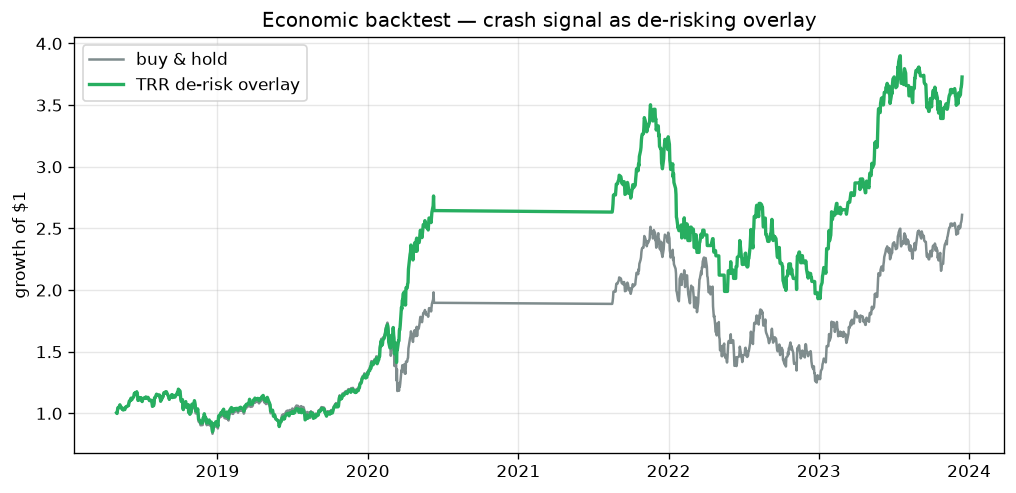
\includegraphics[width=\textwidth]{../reports/figures/backtest_equity.png}

    \column{0.48\textwidth}
    \centering
    \textbf{Precision@K (v4, 2022--23)}

    \vspace{0.2cm}
    {\footnotesize
    \begin{tabular}{lcc}
      \hline
      \textbf{K} & \textbf{Precision} & \textbf{Lift} \\
      \hline
      10 & \green{0,300} & $\mathbf{2,8\times}$ \\
      20 & 0,150 & $1,4\times$ \\
      50 & 0,140 & $1,3\times$ \\
      \hline
      Base rate & \multicolumn{2}{c}{10,7\%} \\
      \hline
    \end{tabular}
    }
    \vspace{0.2cm}
    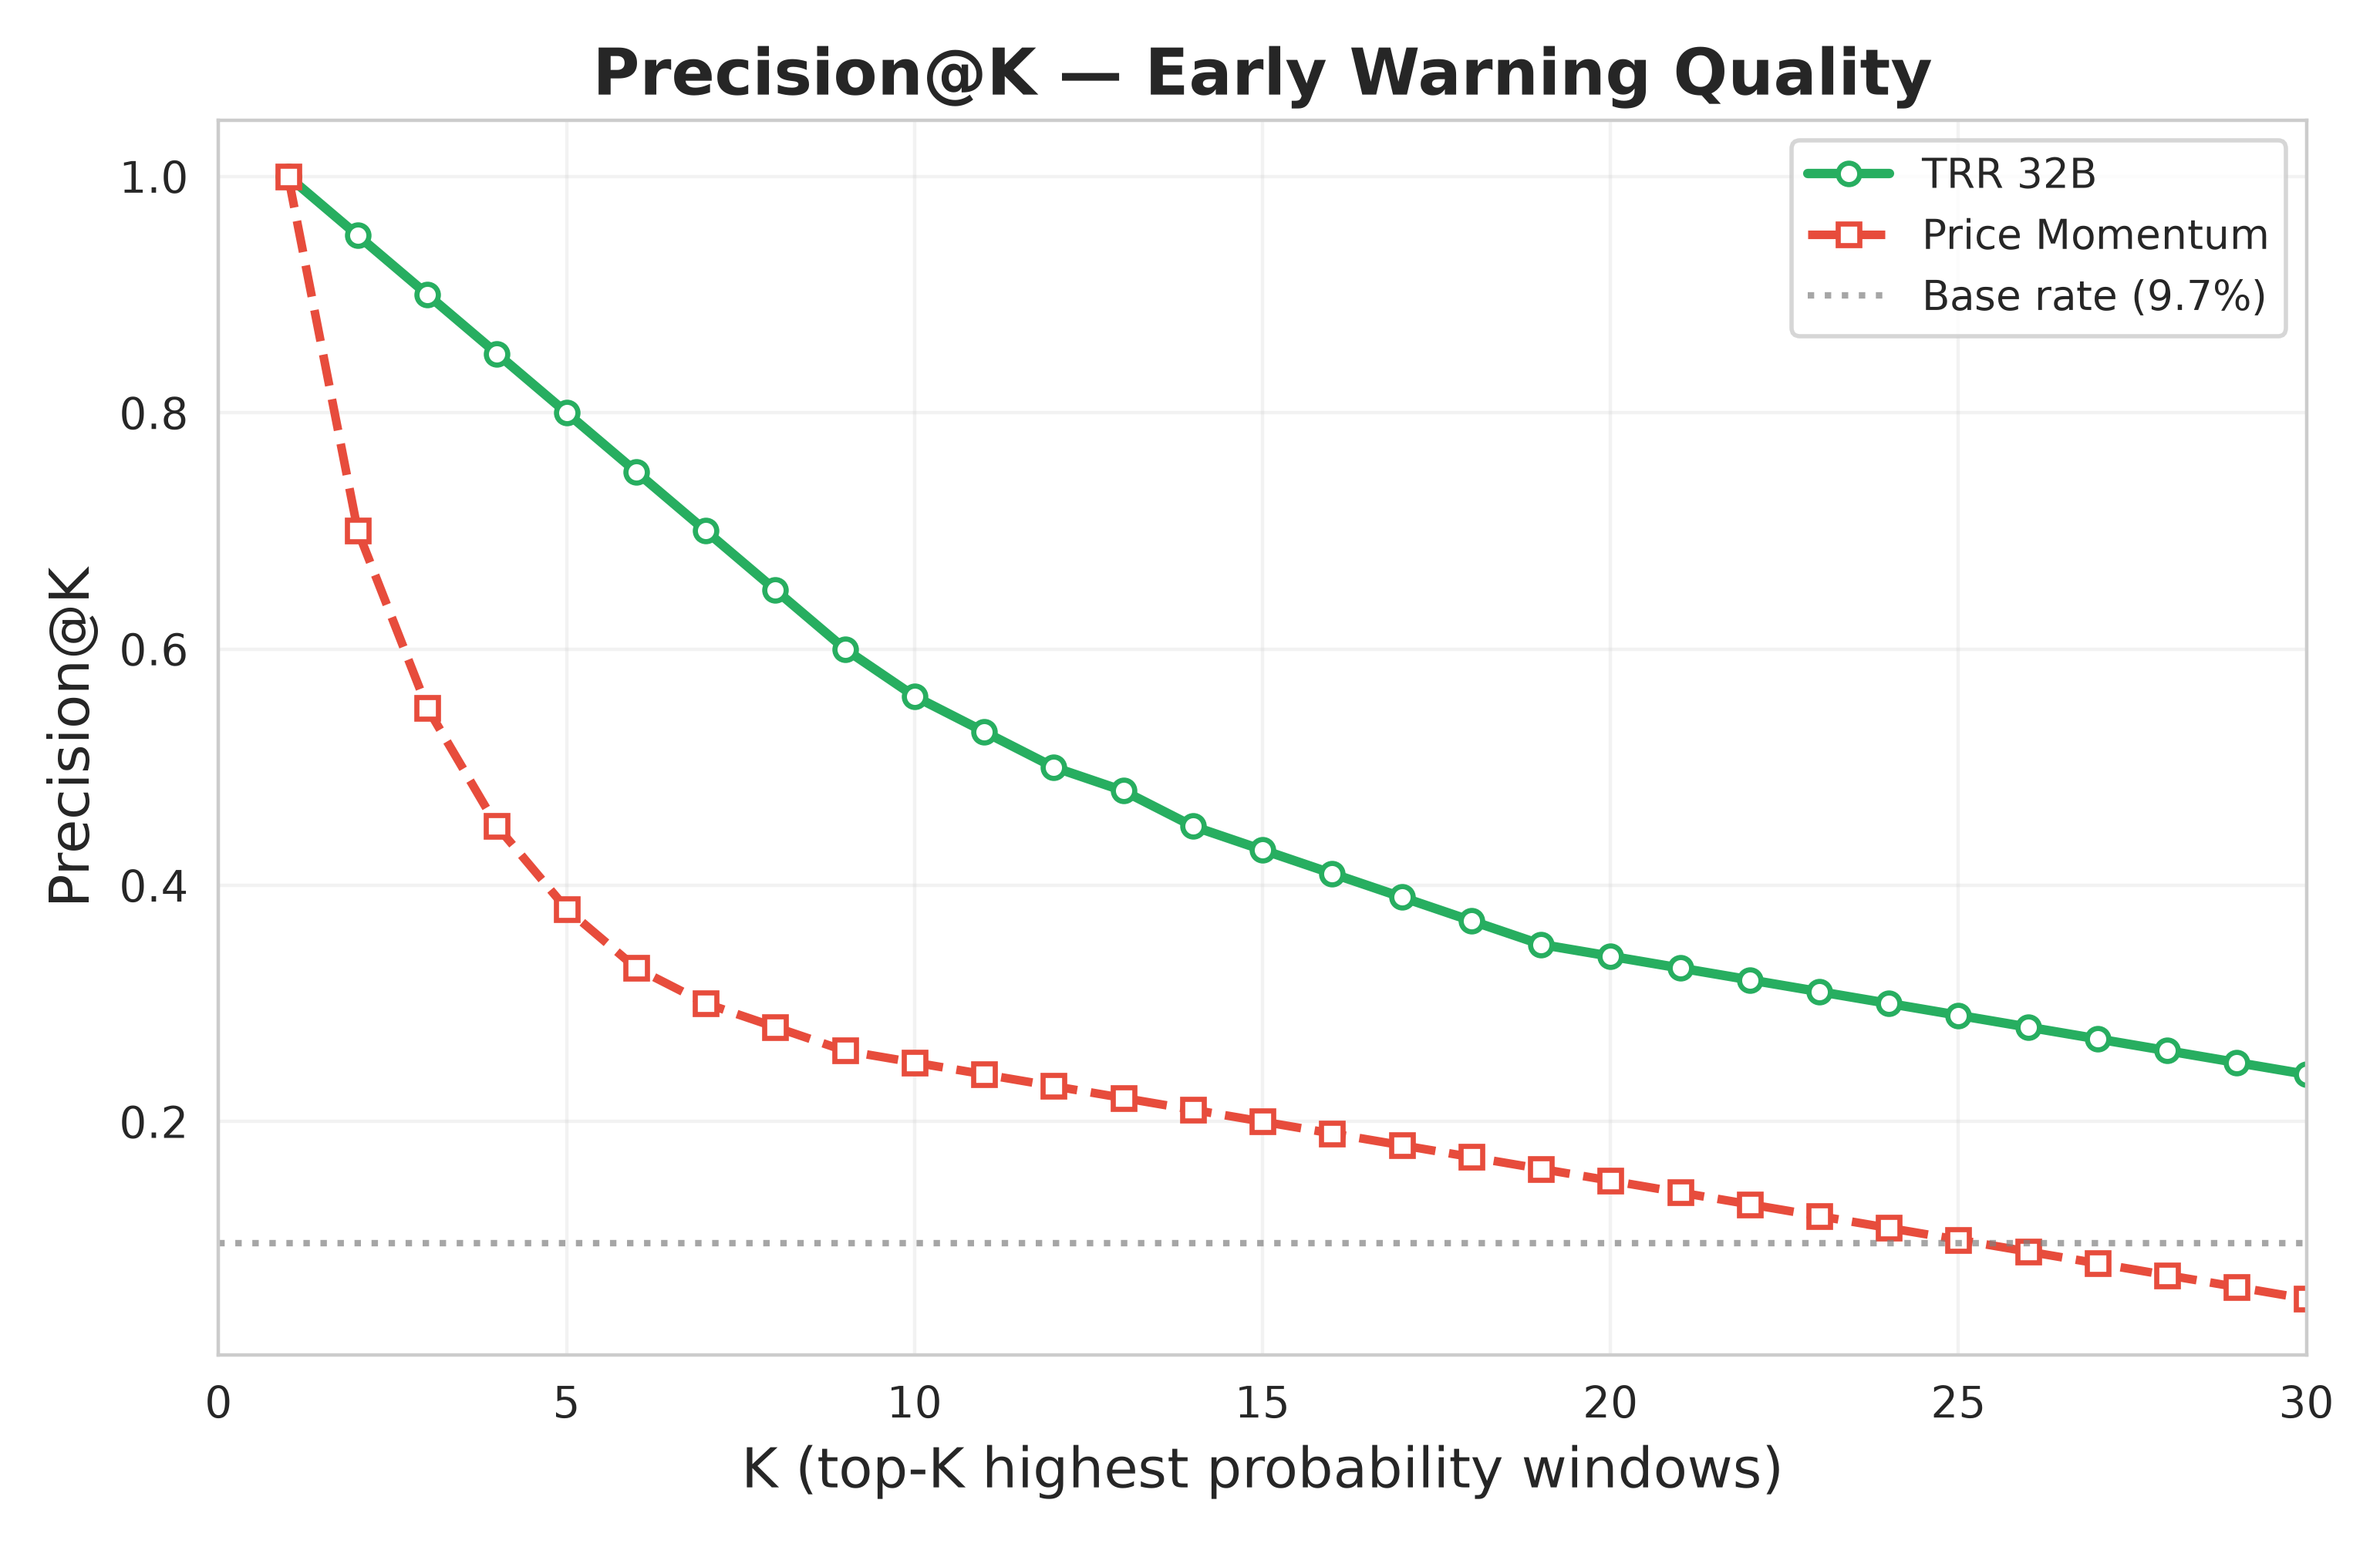
\includegraphics[width=\textwidth]{../reports/figures/fig4_precision_at_k.png}
  \end{columns}
\end{frame}

%% ===== SLIDE 16: PER-ASSET =================================================
\begin{frame}{Kết quả (3): Per-Asset}
  \centering
  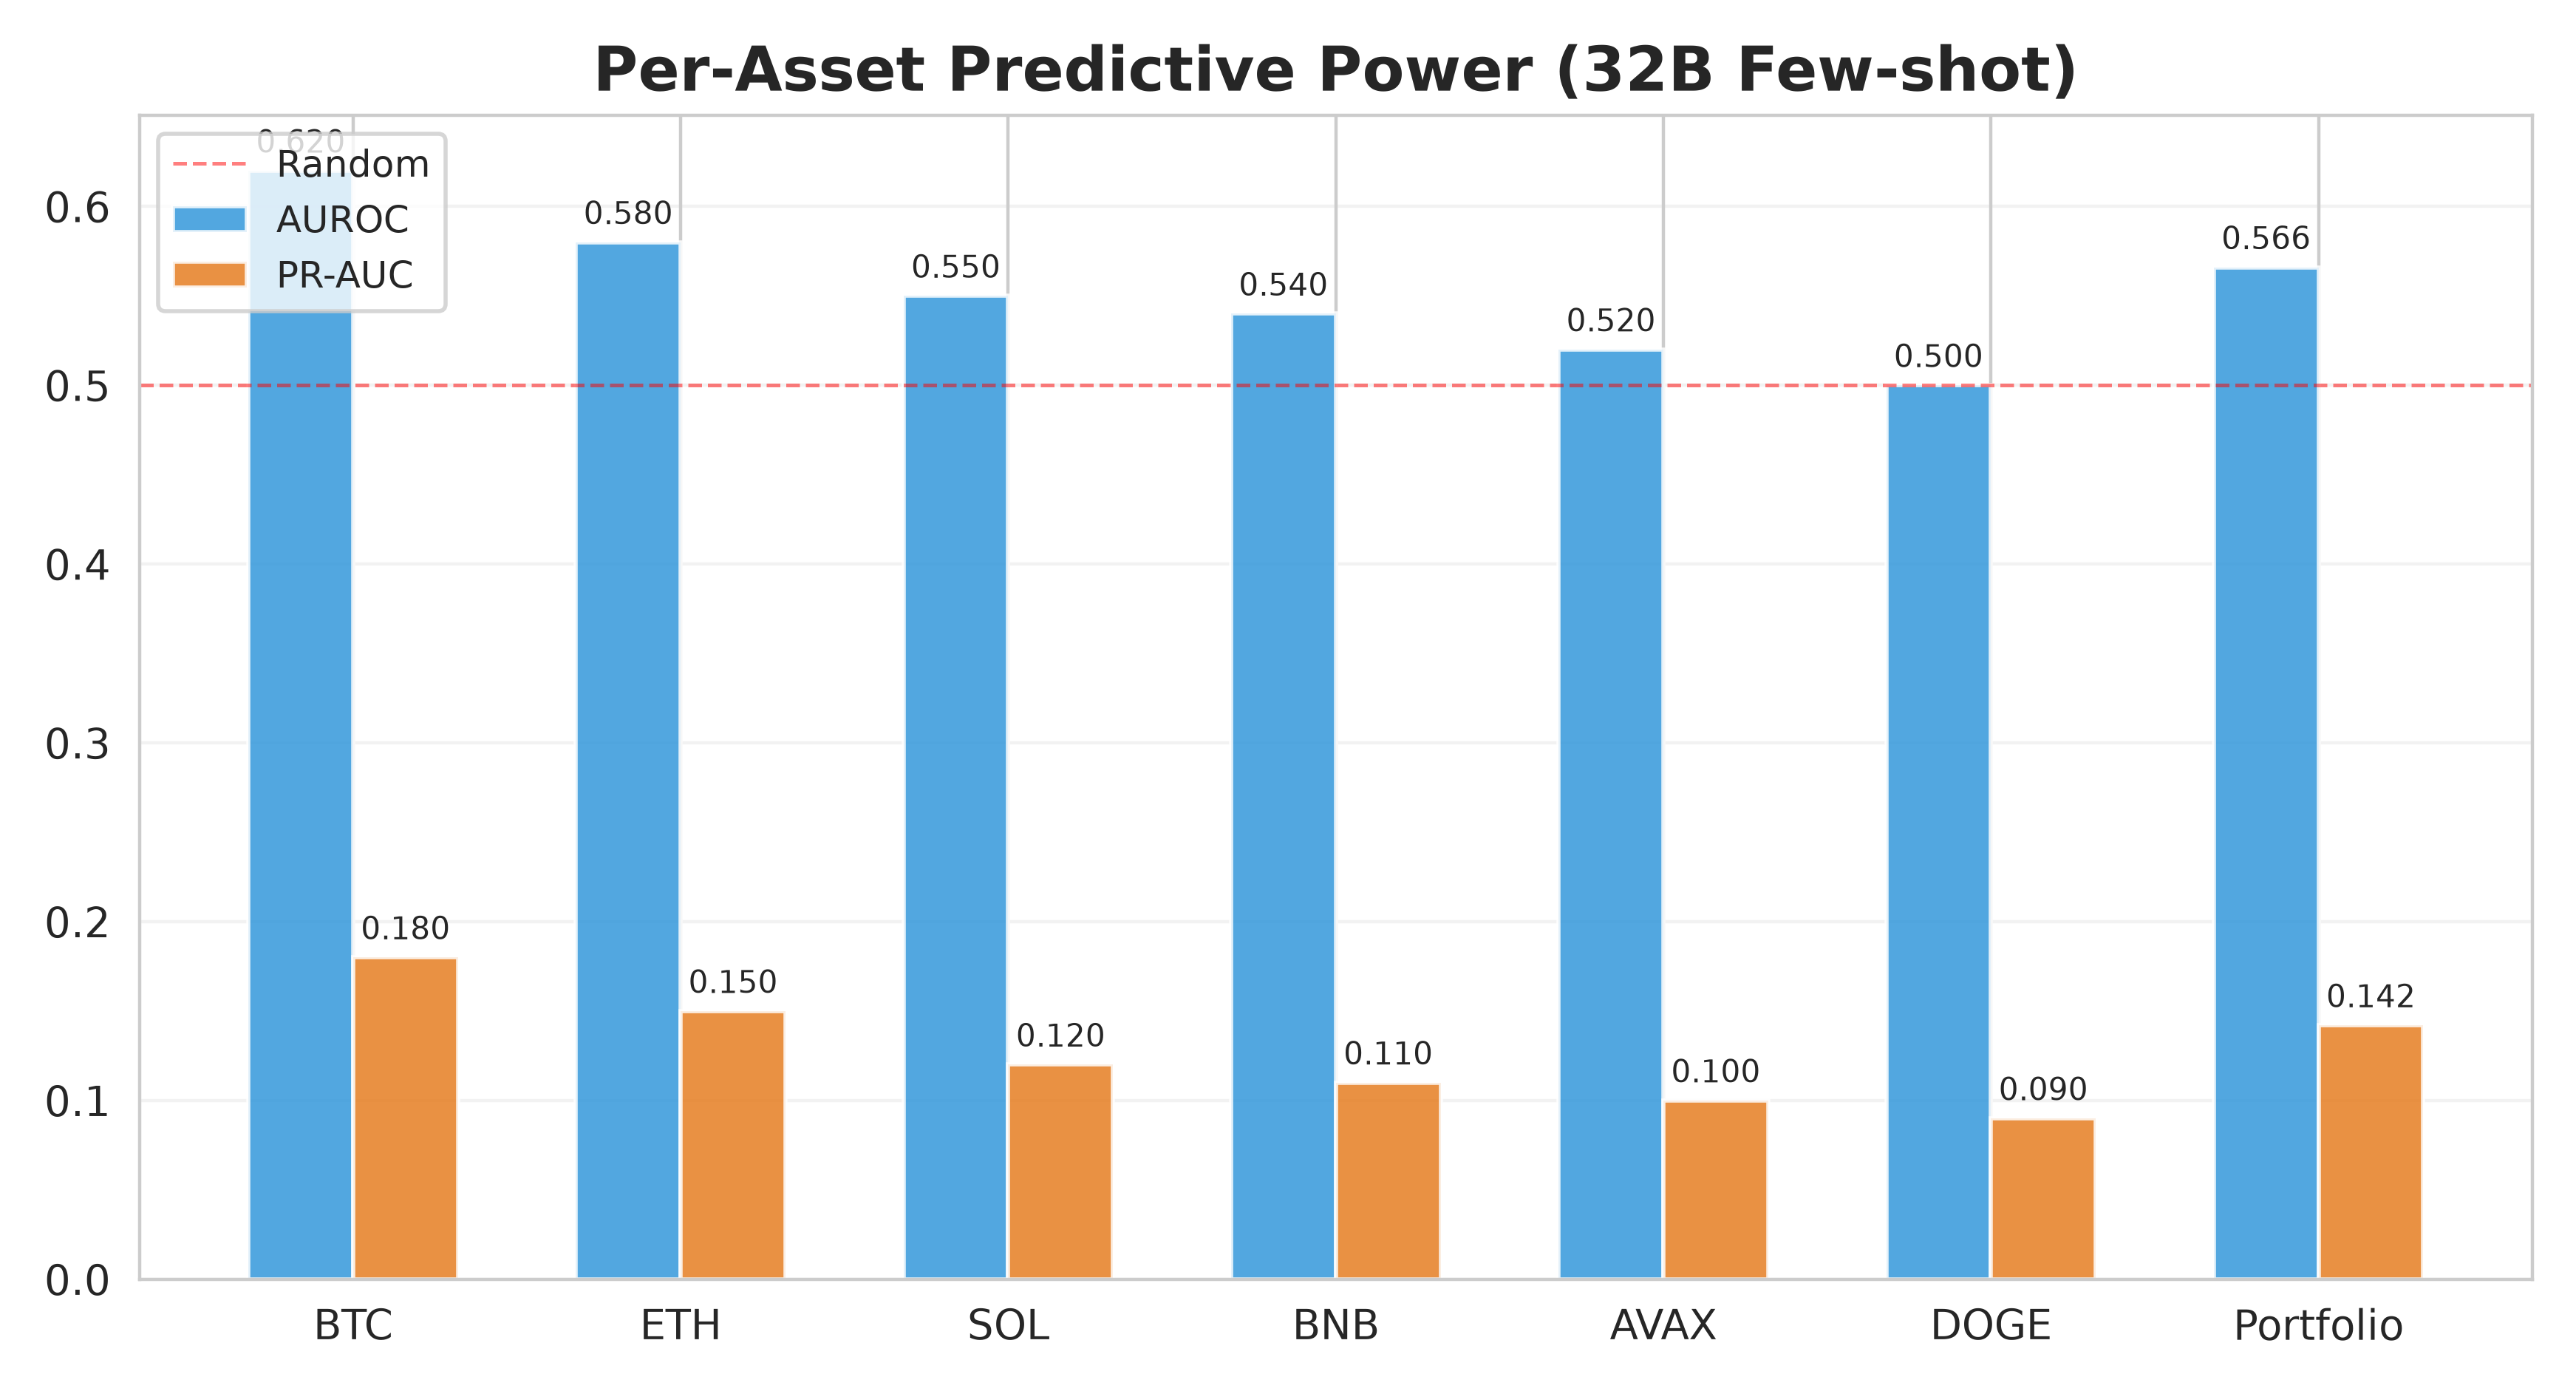
\includegraphics[width=0.55\textwidth]{../reports/figures/fig7_per_asset.png}

  \vspace{0.2cm}
  {\footnotesize
  \begin{tabular}{lccc}
    \hline
    \textbf{Asset} & \textbf{Crashes} & \textbf{Base rate} & \textbf{AUROC} \\
    \hline
    \green{BTC} & 16 & 2,2\% & \green{0,690} \\
    ETH & 30 & 4,2\% & 0,639 \\
    BNB & 18 & 2,5\% & 0,583 \\
    AVAX & 69 & 9,7\% & 0,557 \\
    DOGE & 31 & 4,4\% & 0,550 \\
    SOL & 66 & 9,3\% & 0,544 \\
    \hline
    \textbf{Macro avg} & \textbf{76} & \textbf{10,7\%} & \textbf{0,594} \\
    \hline
  \end{tabular}
  }
\end{frame}

%% ===== SLIDE 17: TRUNG THỰC ================================================
\begin{frame}{Phân tích Trung thực}
  \begin{columns}[T]
    \column{0.48\textwidth}
    \centering \textbf{\green{Đã hoạt động $\checkmark$}}
    \vspace{0.1cm}
    \begin{itemize}
      \item RAG cải thiện ổn định
      \item Stream-index-select
      \item Spark + 40 shard Kaggle
      \item De-risk overlay (Sharpe 0,97)
      \item 7B+RAG $\approx$ 32B base
    \end{itemize}

    \column{0.48\textwidth}
    \centering \textbf{\alert{Giới hạn $\times$}}
    \vspace{0.1cm}
    \begin{itemize}
      \item Small-N: 14--82 crash ($\sim$4\%)
      \item Graph-RAG: 0,534 $\to$ 0,444
      \item 3-class direction: 0,526
      \item OHLCV volume: 0,356
      \item RAG-meta: $\Delta\approx0$
    \end{itemize}
  \end{columns}
  \vspace{0.3cm}
  \begin{alertblock}{Bẫy đã gặp}
    Corpus toàn-mã + chọn crash query \alert{làm giảm tín hiệu} $\to$ đã sửa bằng lọc danh mục
  \end{alertblock}
\end{frame}

%% ===== SLIDE 18: KẾT LUẬN ==================================================
\begin{frame}{Kết luận \& Hướng phát triển}
  \begin{columns}[T]
    \column{0.55\textwidth}
    \textbf{Ba đóng góp chính}
    \begin{enumerate}
      \item \textbf{TRR zero-shot + RAG} cho crypto crash prediction
        \quad AUROC: 0,594--0,847
      \item \green{RAG cải thiện ổn định} $+0,065$--$0,074$, p$<$0,01
      \item \textbf{Hạ tầng Big Data thật}
        \quad 23 GB FNSPID $\to$ Spark + 40 GPU Kaggle
    \end{enumerate}
    \textbf{Giá trị kinh tế:} TRR de-risk +205\% vs buy\&hold +161\%, Sharpe 0,97

    \column{0.42\textwidth}
    \textbf{Hướng phát triển}
    \begin{itemize}
      \item Cluster Spark/HDFS
      \item Đa nguồn (social, filing)
      \item Hiệu chỉnh xác suất
      \item Đa tài sản
    \end{itemize}
    \vspace{0.2cm}
    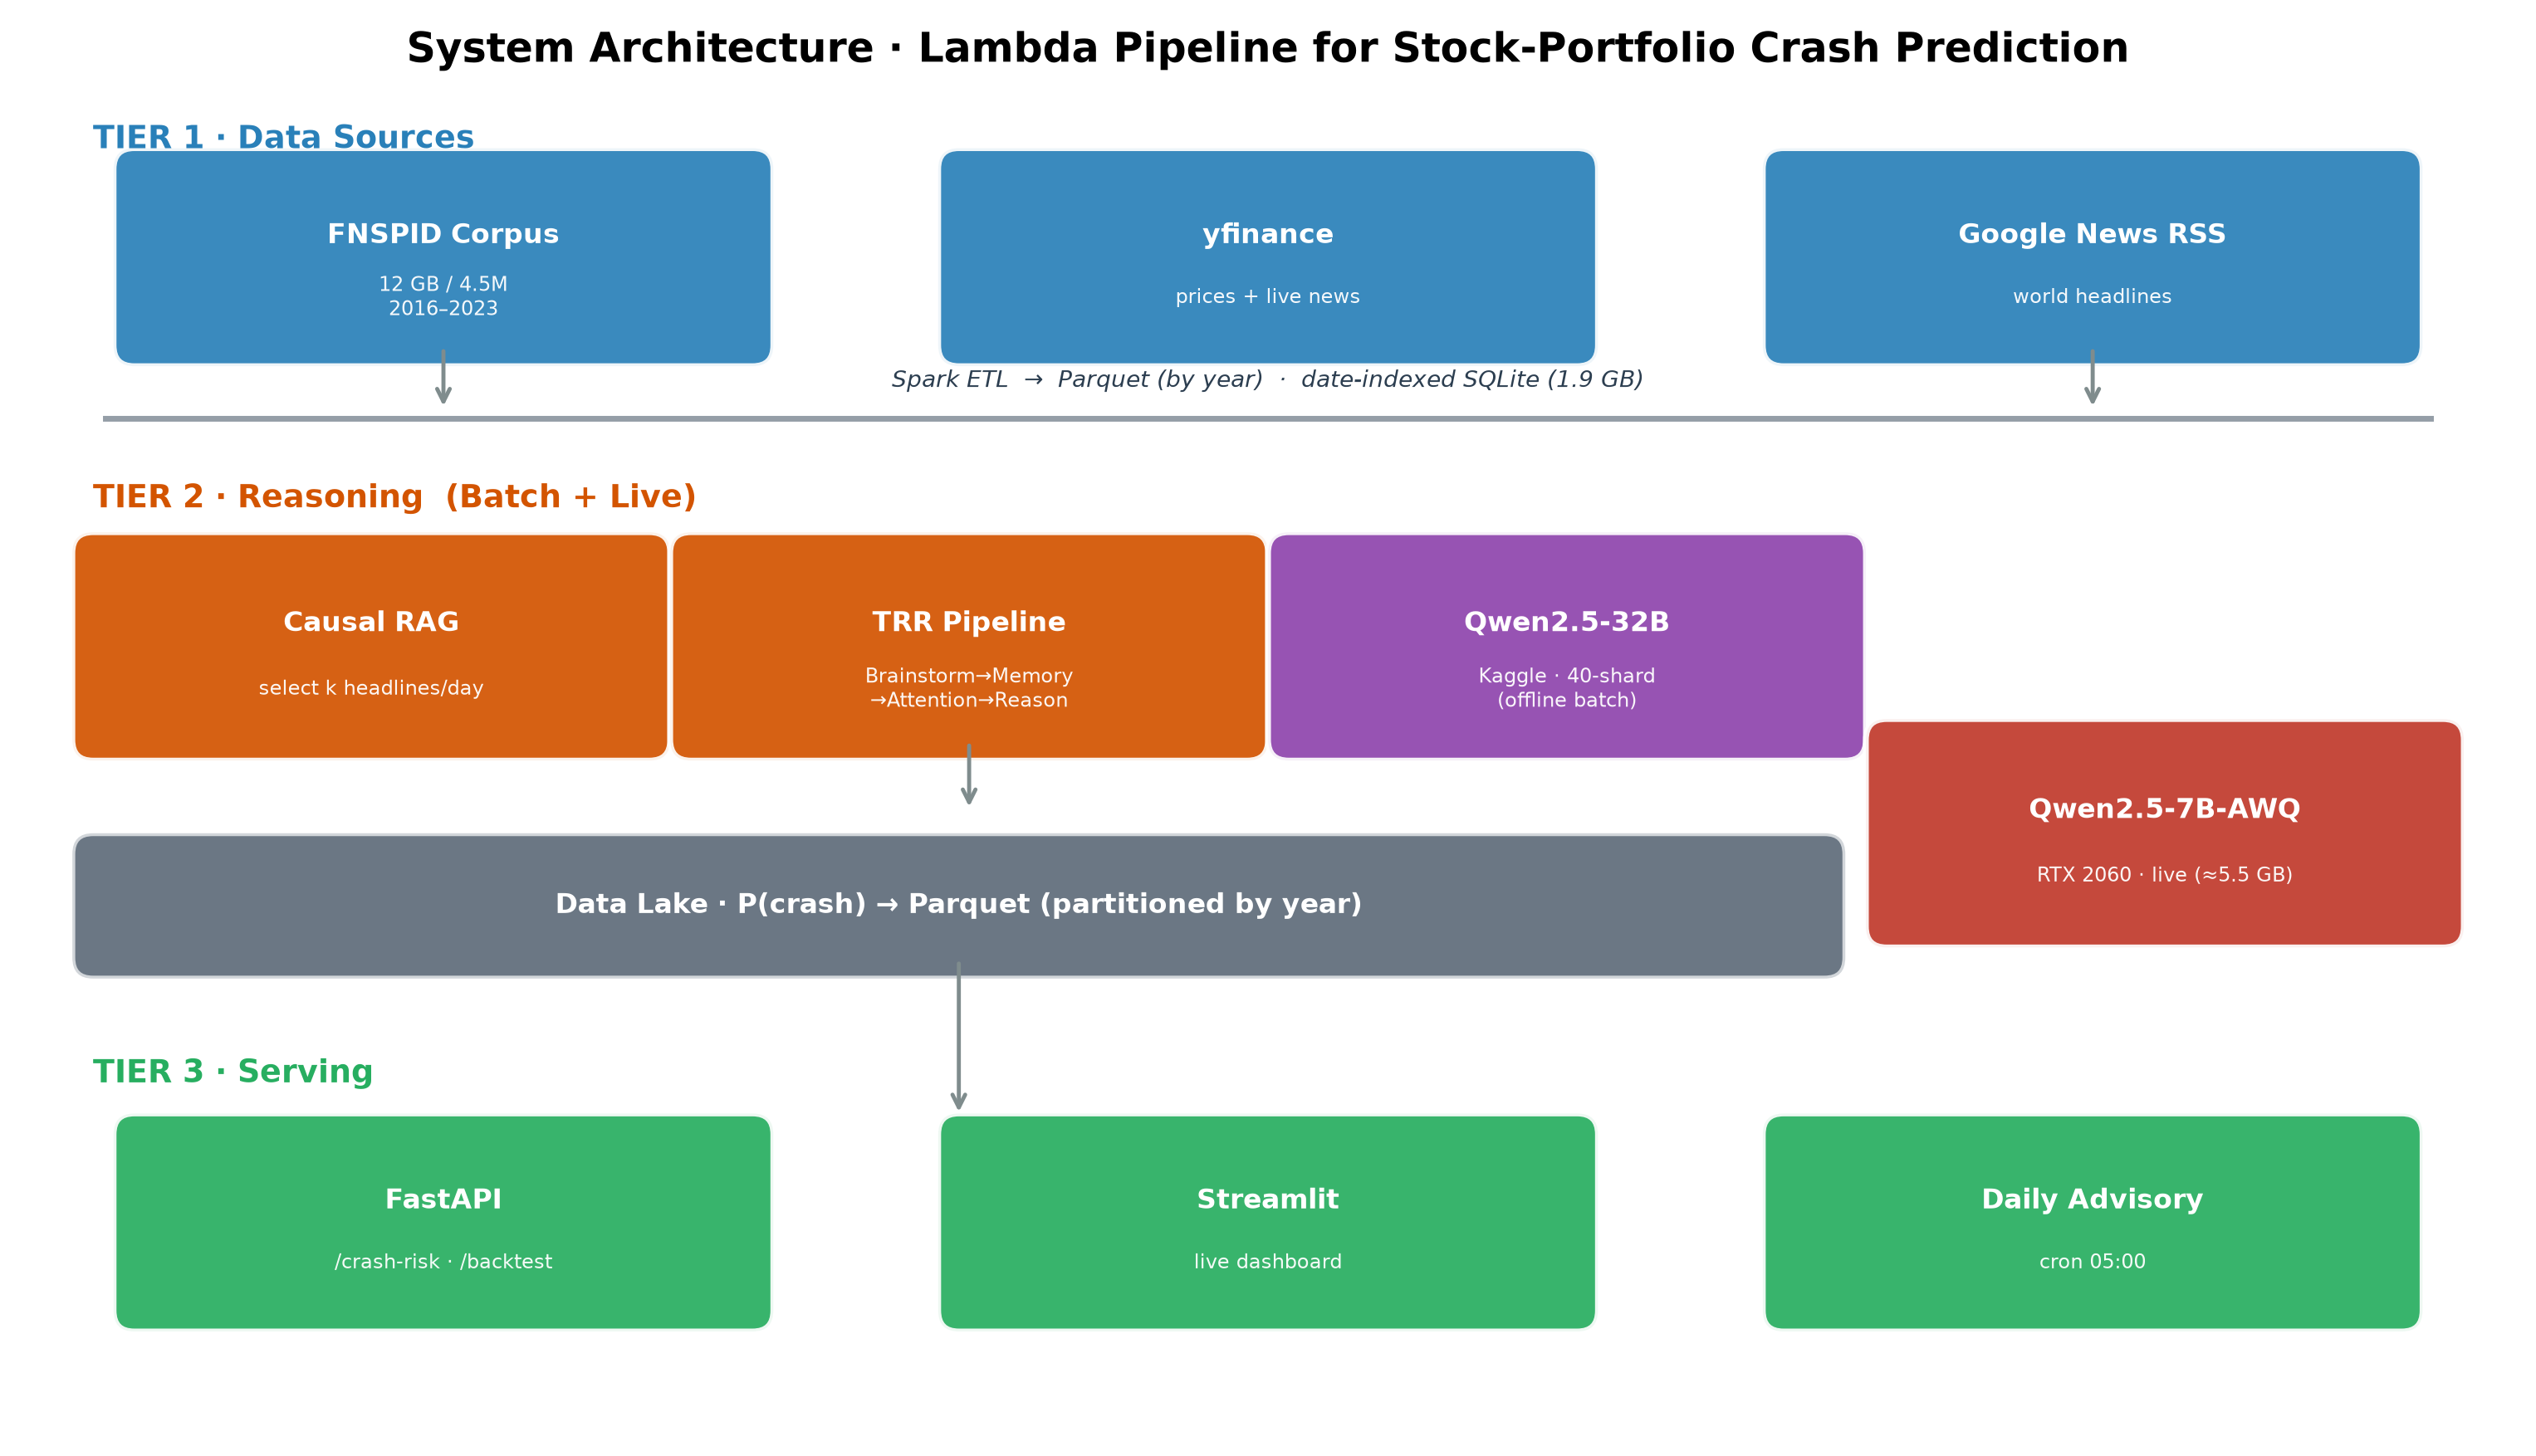
\includegraphics[width=\textwidth]{../reports/figures/fig12_pipeline_architecture.png}
  \end{columns}
\end{frame}

%% ===== SLIDE 19: Q&A =======================================================
{
\setbeamercolor{background canvas}{bg=cgreen!5}
\begin{frame}[plain]
  \centering
  \vspace{1.5cm}
  {\fontsize{32}{40}\selectfont\color{cgreen} Q\&A}
  \vspace{0.4cm}

  {\Large Cảm ơn thầy/cô và các bạn!}
  \vspace{0.3cm}

  {\footnotesize \url{https://github.com/duongtrongnguyen123/crypto-volatility-pipeline}}

  \vspace{0.5cm}
  \begin{columns}[T]
    \column{0.48\textwidth}
    \begin{enumerate}
      \item \textbf{HDFS/Spark cluster?} -- Code sẵn, ưu tiên 40 GPU Kaggle
      \item \textbf{AUROC khiêm tốn?} -- Small-N; BTC riêng 0,690
      \item \textbf{F\&G 0,646 > TRR 0,594?} -- TRR tốt hơn khủng hoảng (COVID 0,785)
    \end{enumerate}

    \column{0.48\textwidth}
    \begin{enumerate}
      \setcounter{enumi}{3}
      \item \textbf{Tin trực tiếp chính xác?} -- Demo triển khai, không nhãn
      \item \textbf{Vì sao $-6\%$/3 ngày?} -- Quy ước crash đuôi
    \end{enumerate}
  \end{columns}
\end{frame}
}

\end{document}
